\documentclass[11pt,a4paper]{article}
\usepackage[review]{acl}
\usepackage{times}
\usepackage{latexsym}
\usepackage{amsmath}
\usepackage{amssymb}
\usepackage{graphicx}
\usepackage{booktabs}
\usepackage{xcolor}
\usepackage{multirow}
\usepackage{placeins}
\renewcommand{\UrlFont}{\ttfamily\small}

\usepackage{microtype}

\setcounter{topnumber}{1}
\setcounter{dbltopnumber}{1}
\setcounter{totalnumber}{2}
\renewcommand{\topfraction}{0.9}
\renewcommand{\dbltopfraction}{0.9}
\renewcommand{\textfraction}{0.07}
\renewcommand{\floatpagefraction}{0.8}
\renewcommand{\dblfloatpagefraction}{0.8}

%\aclfinalcopy % Uncomment this line for the final submission
%\def\aclpaperid{***} %  Enter the acl Paper ID here

\newcommand\BibTeX{B\textsc{ib}\TeX}

\title{When Is Random Dimension Selection Enough? Training Paradigm and Compression Level Are Associated with the Value of Task-Aware Pruning}

\author{First Author \\
  Affiliation / Address line 1 \\
  Affiliation / Address line 2 \\
  Affiliation / Address line 3 \\
  \texttt{email@domain} \\\And
  Second Author \\
  Affiliation / Address line 1 \\
  Affiliation / Address line 2 \\
  Affiliation / Address line 3 \\
  \texttt{email@domain} \\}

\date{}

\begin{document}
\maketitle


%TODO: 摘要引言综合两版内容
\begin{abstract}
Modern text embedding models produce high-dimensional vectors that are expensive to store and compare at scale. We study post-hoc compression for frozen, off-the-shelf embedding models and ask: \emph{when are task-aware gains over random large enough to justify their cost?} Across 11 models and 34 MTEB tasks, we find that the answer varies sharply by model's \textbf{training paradigm} and compression level. For \emph{Retrieval-optimized Embedders} and most \emph{Instruction-Conditioned Embedders}, random selection is a strong baseline: at 256 retained dimensions, even an optimized oracle with full access to evaluation data improves by only $+2.4$--$5.3\%$. In contrast, Roberta-InBedder and \emph{General-purpose Language Model Backbones} show substantially larger gains of $+8.2$--$11.8\%$ from task-aware selection. Magnitude-based pruning, despite being a natural zero-cost heuristic, matches or underperforms random selection. Cross-task transfer performs almost identically to random selection, exceeding random by only $+0.8\%$ at dim=256. Stronger baselines such as gradient saliency, activation variance, and learned masks offer marginal gains for Retrieval-optimized Embedders and may even harm General-purpose Language Model Backbones. These patterns can be explained by near-uniform chunk-level importance. Random selection is therefore a strong baseline for moderate post-hoc compression, while task-aware selection is most useful under aggressive compression or for General-purpose Language Model Backbones.
\end{abstract}

%引言综合两版内容
\section{Introduction}

%图注要改!
\begin{figure*}[!t]
    \centering
    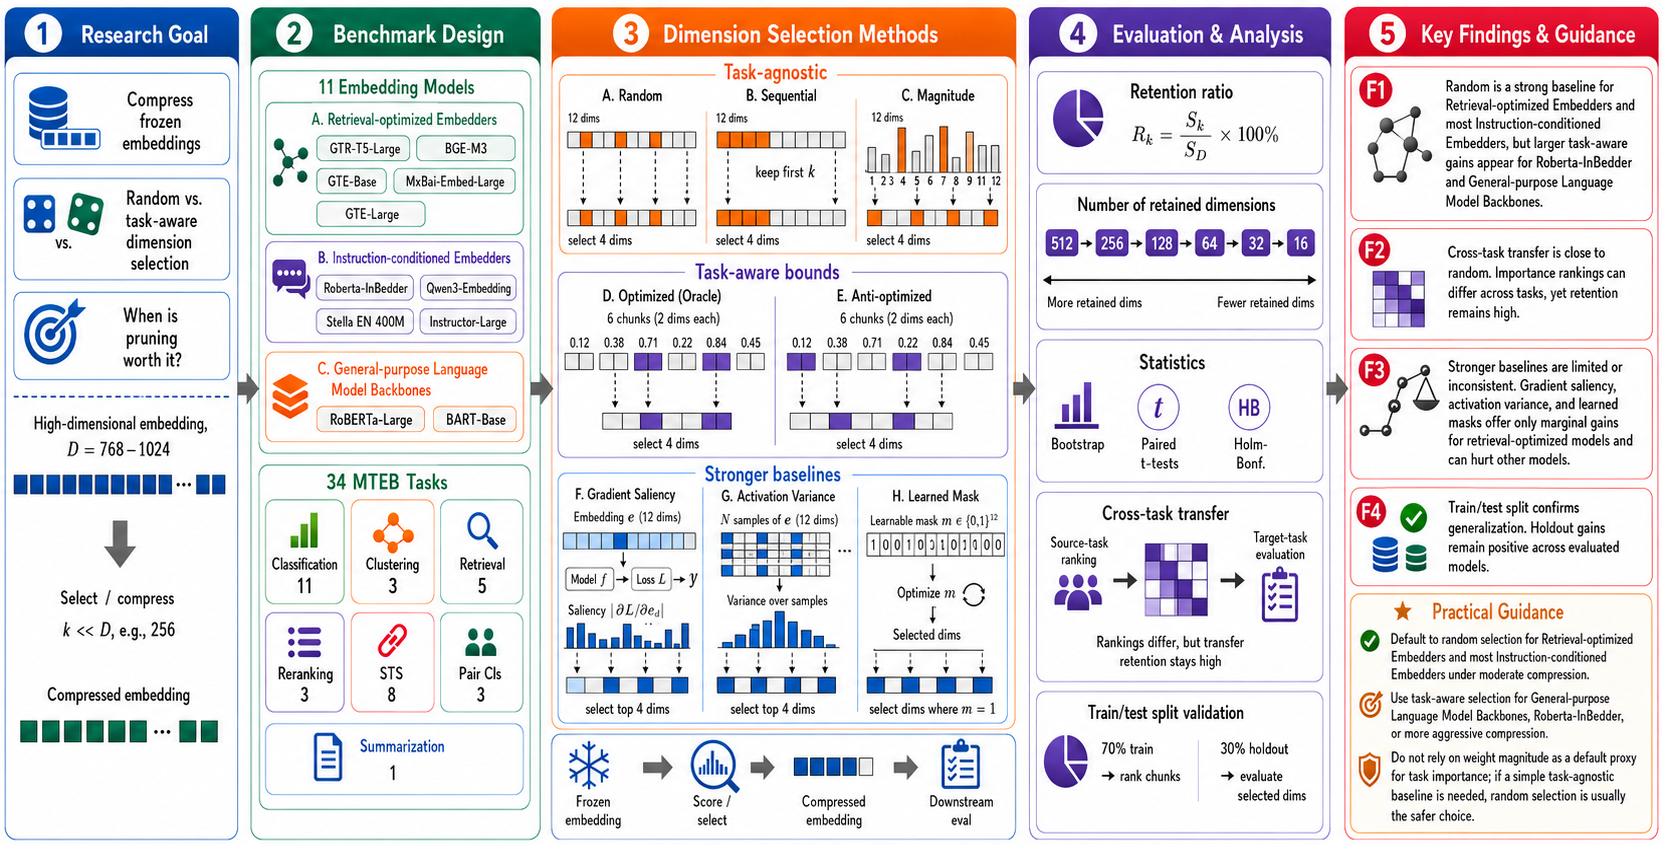
\includegraphics[width=0.95\linewidth]{figures/fig_concept_overview.png}
    \caption{Research framework overview. We evaluate 8 dimension selection methods across 11 text embedding models and 34 MTEB tasks: task-agnostic baselines (Random, Sequential, Magnitude), task-aware bounds (Optimized and Anti-optimized), and stronger baselines (Gradient Saliency, Activation Variance, and Learned Mask). Evaluation is based on retention ratio over different retained dimensionalities, with bootstrap confidence intervals and paired significance tests. Train/test split validation and cross-task transfer analysis are also conducted. The final panel summarizes the main empirical findings and practical guidance for post-hoc embedding compression.}
    \label{fig:concept_overview}
\end{figure*}

Dense text embeddings now sit inside many NLP systems, powering semantic search, clustering, classification, and reranking. State-of-the-art models produce vectors with 768–4096 dimensions. Since storage and similarity computation both grow linearly with dimension, these vectors become costly when a system must process millions or billions of tokens. Motivated by this cost, \citet{takeshita2025randomly} show that randomly removing 50\% of dimensions from modern embeddings typically causes only a 5--10\% drop in retrieval and classification accuracy. \citet{tsukagoshi2025redundancy} report that prompt-based LLM embeddings still work well even after retaining only 25\% of dimensions. These findings suggest \textbf{useful signal is broadly distributed} across dimensions, rather than concentrated in a small subset. 

We revisit this observation with a narrower question: \emph{when are task-aware gains over random large enough to justify their cost?} This question has direct practical implications. If random selection is sufficient, then post-hoc embedding compression requires no task-specific evaluation. If task-aware selection provides substantial gains, then investing in importance estimation is worthwhile. We test this question on 11 embedding models and 34 MTEB tasks, comparing 8 dimension selection strategies. The answer, we show, depends on \emph{training paradigm} and compression level: Retrieval-optimized Embedders and most Instruction-conditioned Embedders produce near-uniform importance at moderate compression where random is hard to beat, while General-purpose Language Model Backbones exhibit more exploitable structure. Figure~\ref{fig:concept_overview} summarizes our research framework and key findings.

Our contributions are:
\begin{enumerate}
    \item We provide a broad evaluation of post-hoc dimension selection for frozen text embeddings across 11 models and 34 MTEB tasks, quantifying when optimized selection provides sufficient gains over random selection to justify its additional cost.
    \item We probe its boundary conditions with complementary experiments, showing that stronger baselines on dimension selection provide limited or inconsistent gains, and that the observed association with training paradigm persists under held-out validation.
    \item We identify nearly uniform chunk importance as an explanation for small optimized--random gap among Retrieval-optimized Embedders and most Instruction-conditioned Embedders.
\end{enumerate}

\section{Related Work}

\paragraph{Embedding redundancy.}
Several recent works have examined the redundancy of text embeddings. \citet{takeshita2025randomly} evaluate 6 models on retrieval and classification tasks and find that randomly removing 50\% of dimensions causes minor accuracy drops. \citet{tsukagoshi2025redundancy} study prompt-based LLM embeddings and show that classification and clustering can tolerate extreme pruning ($>$99.5\% dimension removal), while retrieval needs more dimensions. \citet{zhang2024evaluating} compare unsupervised dimensionality reduction methods, showing PCA can halve embedding size with little loss. Our work extends these findings by measuring when and to what extent task-specific optimized selection outperforms random baselines.

\paragraph{Task-aware embedding compression.}
Several methods try to exploit task-specific dimension importance. \citet{matryoshka-adaptor} learn lightweight adaptors that restructure LLM embeddings. \citet{dime2025} estimate per-dimension importance for dense retrieval. \citet{smec2025} combine Matryoshka representation learning with adaptive dimension selection. \citet{gaprune2025} use gradient alignment for domain-specific pruning. \citet{beyond-matryoshka2025} relax contiguous-dimension constraint via sparse coding. These methods typically require retraining. For reference, we include stronger deployable baselines (gradient saliency, activation variance, learned masks) in our experiments. 

%TODO: 可以结合新版的，多展示一些模型
\begin{figure*}[t]
    \centering
    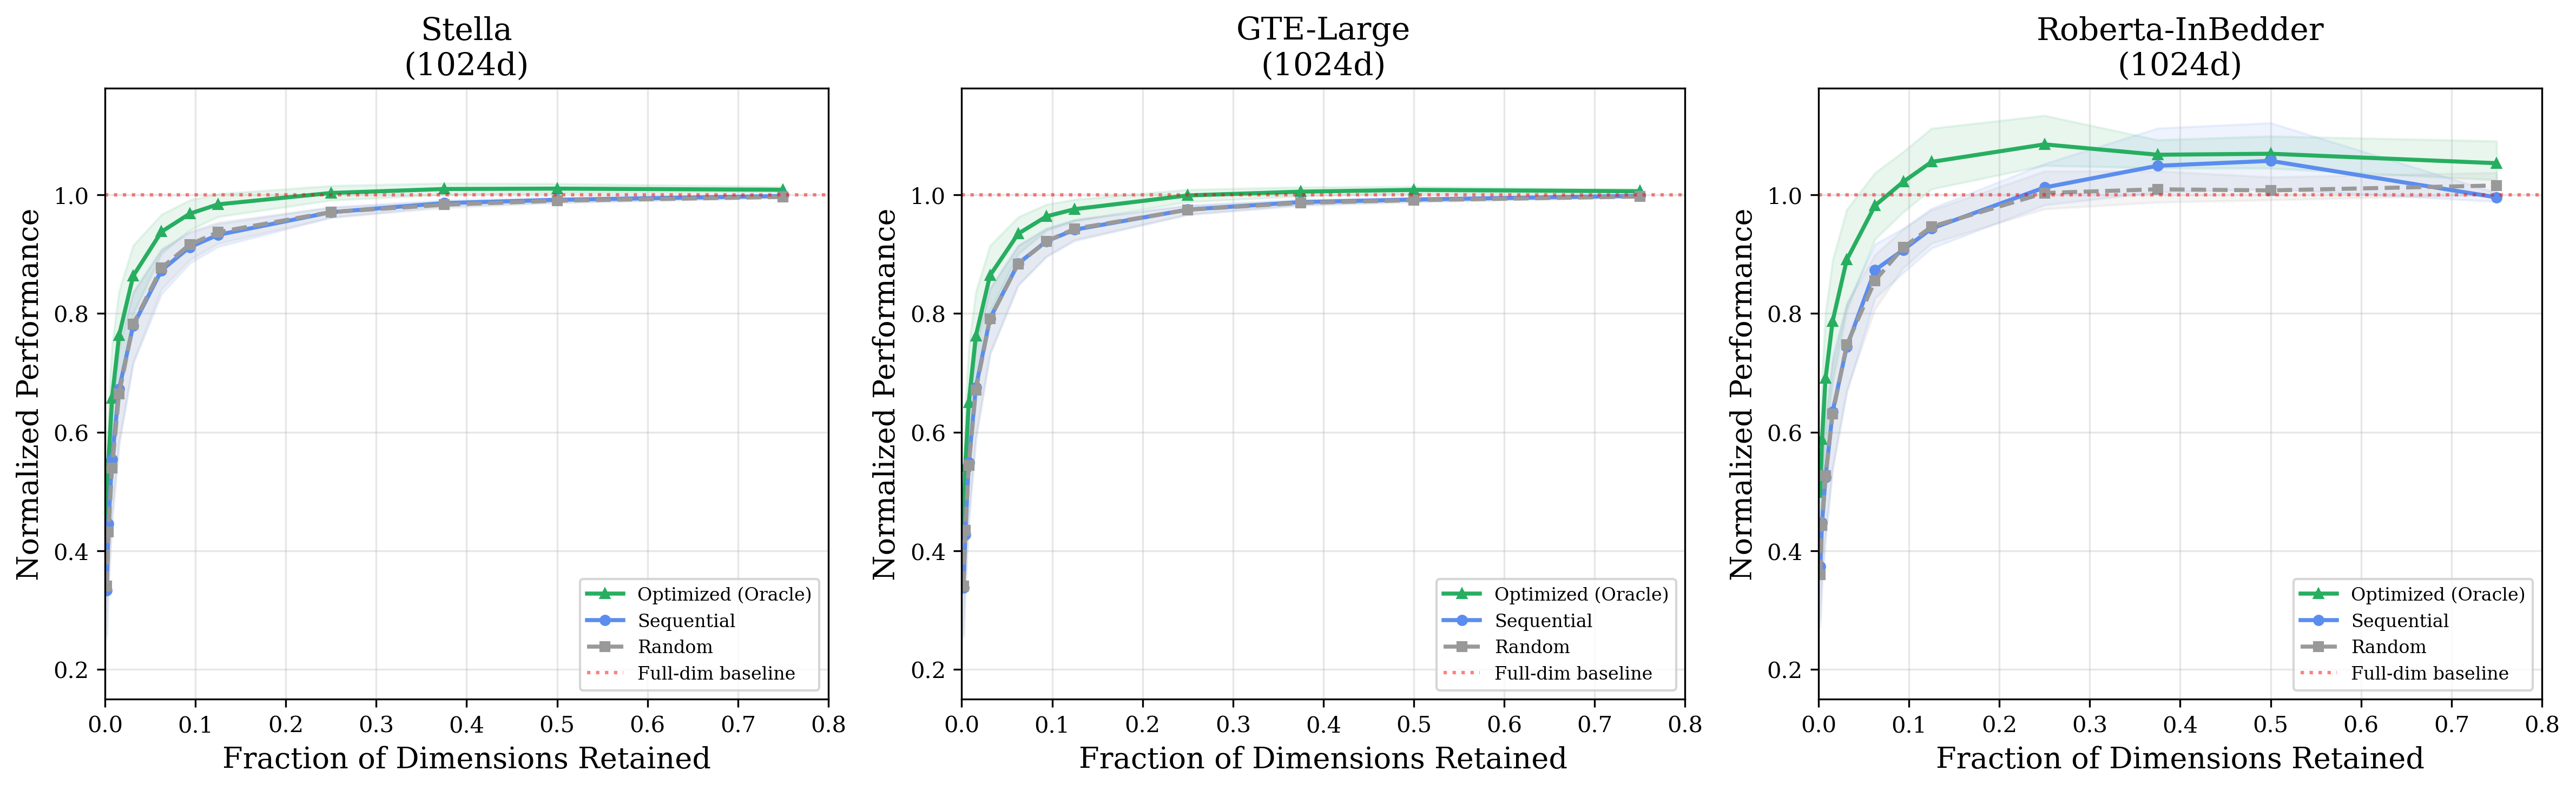
\includegraphics[width=0.95\linewidth]{figures/fig6_pruning_ratio_sweep.png}
    \caption{Retention ratio as a function of the fraction of dimensions retained for three representative models. Optimized (green) consistently exceeds Random (gray), while Sequential (blue) closely tracks Random throughout. The optimized--random gap remains modest for GTE-Large and Stella across retention levels, and is notably larger for Roberta-InBedder. Shaded bands show 95\% bootstrap confidence intervals over tasks.}
    \label{fig:pruning_ratio_sweep}
\end{figure*}

\paragraph{Matryoshka representation learning.}
\citet{matryoshka2023} train embeddings where the first $k$ dimensions are optimized to be a good representation at any truncation level, showing that a useful prefix ordering can be learned through training. Our sequential selection baseline directly tests whether off-the-shelf models already exhibit Matryoshka-like properties.

\paragraph{Neural network pruning.}
The broader pruning literature \citep{han2015pruning,lottery-ticket,structured-pruning} show that many trained weights are redundant and can be removed. However, these methods usually rely on iterative retraining. We study a different setting: pruning \emph{output embeddings} of frozen models, with no retraining or fine-tuning.

\paragraph{Intrinsic dimensionality.}
\citet{li2018measuring} and \citet{alemohammad2023intrinsic} show that neural network representations live on low-dimensional manifolds. Our entropy analysis complements this by measuring \emph{uniformity} of per-dimension importance.

\section{Methodology}
\label{sec:method}
\subsection{Models and Tasks}

\paragraph{Models.}
%模型分类名称要修改!
We evaluate 11 text embedding models with diverse architectures and training objectives. For clarity, we group them into three families. First are \emph{General-purpose Language Model Backbones} not originally designed as embedding models: RoBERTa-Large \citep{roberta} (1024-d) and BART-Base \citep{bart} (768-d). Second are \emph{Instruction-conditioned Embedders}, whose embedding ability is added or strengthened through post-training adaptation: Roberta-InBedder \citep{inbedder} (1024-d), Qwen3-Embedding \citep{qwen3-embedding} (1024-d), Stella EN 400M \citep{stella}, and Instructor-Large \citep{instructor} (768-d). Third are \emph{Retrieval-optimized Embedders}, which are trained directly for retrieval-style representation learning: GTR-T5-Large (768-d), BGE-M3 \citep{bge} (1024-d), GTE-Base (768-d), MxBai-Embed-Large (1024-d), and GTE-Large \citep{gte} (1024-d).
Stella is released with linear heads for multiple output sizes (512--8192). We use its default 1024-dimensional head before applying post-hoc dimension selection. Appendix Table~\ref{tab:model_list} summarizes which evaluations are available for each model.

\paragraph{Tasks.}
We use 34 MTEB tasks \citep{mteb} covering classification (11 tasks), clustering (3 tasks), retrieval (5 tasks), reranking (3 tasks), STS (8 tasks), pair classification (3 tasks), and summarization (1 task). Table~\ref{tab:per_task_gte} lists the specific tasks included in our evaluation.

\subsection{Dimension Selection Methods}

Given a $D$-dimensional embedding $\mathbf{e} \in \mathbb{R}^D$ and a target dimensionality $k < D$, we compare five ways to choose which dimensions to retain:

\paragraph{1. Random.}
Uniformly sample $k$ of $D$ dimensions without replacement, producing a $k$-dimensional subvector. We repeat this 10 times with different random seeds and report the mean score:
\begin{equation}
\mathbf{e}^{(\text{rand})} = \mathbf{e}[\mathcal{I}_k], \quad \mathcal{I}_k \sim \mathrm{Uniform}\big(\{1,\ldots,D\}, k\big)
\end{equation}
where $\mathcal{I}_k \subset \{1, \ldots, D\}$ is a random index set of size $k$, and $\mathbf{e}[\mathcal{I}_k]$ denotes the resulting subvector.

\paragraph{2. Sequential.}
Retain the first $k$ dimensions in the model's original output order:
\begin{equation}
\mathbf{e}^{(\text{seq})} = \mathbf{e}[1:k] = (e_1, e_2, \ldots, e_k)
\end{equation}
where $e_i$ denotes the $i$-th component of the embedding vector. This tests whether the native dimension order already encodes importance information.

\paragraph{3. Magnitude.}
Rank dimensions by their L2 norm in the embedding weight matrix $\mathbf{W} \in \mathbb{R}^{V \times D}$, where $V$ is the vocabulary size and $D$ is the embedding dimension:
\begin{equation}
\mathrm{Importance}(d) = \|\mathbf{w}_d\|_2, \quad \mathbf{w}_d = \mathbf{W}[:, d] \in \mathbb{R}^V
\end{equation}
where $\mathbf{w}_d$ is the $d$-th column of the embedding matrix. We then retain the $k$ dimensions with the largest magnitudes. Weight magnitude is a standard pruning heuristic \citep{han2015pruning} since larger weights often indicate greater neuron importance. We use it here to test whether that intuition also works for \emph{output embedding} dimensions. 

\begin{table}[t]
    \centering
    \caption{Summary of the five dimension selection strategies evaluated. ``Task-aware'' indicates whether the method requires task-specific evaluation to construct the dimension ranking. $N = D/w$ is the number of chunks and $|\mathcal{T}|$ is the number of evaluation tasks.}
    \label{tab:methods_summary}
    \small
    \resizebox{\columnwidth}{!}{%
    \begin{tabular}{llcc}
        \toprule
        Method & Selection Criterion & Task-aware? & Cost \\
        \midrule
        Random & Uniform sampling (10 trials) & No & Zero \\
        Sequential & First $k$ dimensions (intrinsic order) & No & Zero \\
        Magnitude & Highest L2 weight norm per dim. & No & Zero \\
        Optimized & Highest chunk-level task score & Yes & $O(N \cdot |\mathcal{T}|)$ \\
        Anti-opt. & Lowest chunk-level task score & Yes & $O(N \cdot |\mathcal{T}|)$ \\
        \bottomrule
    \end{tabular}%
    }
\end{table}

\paragraph{4. Optimized (Oracle).}
Divide the $D$ dimensions into $N = D/w$ contiguous chunks of size $w$ (we primarily use $w = 2$ to balance detail and cost, and further evaluate sensitivity to chunk size in Appendix~\ref{sec:chunk_size}). For each chunk $i$, we measure its standalone contribution by keeping only that chunk and evaluating it on the target task:
\begin{equation}
S_i^T = \mathrm{Eval}(\mathbf{e}[\text{chunk}_i],\; T)
\end{equation}
Rank chunks by $S_i^T$ and retain the top $k/w$ chunks. This gives an \emph{oracle upper bound} on task-aware selection because it is allowed to inspect full task evaluation scores directly.

\paragraph{5. Anti-optimized.}
Same as Optimized, but select the \emph{lowest}-ranked chunks. This establishes a lower bound, showing the worst-case performance when the least informative dimensions are kept.

Table~\ref{tab:methods_summary} summarizes all five strategies. The first three (Random, Sequential, Magnitude) are \emph{task-agnostic}: they need no task-specific evaluation and can be applied directly to any frozen model. The last two (Optimized, Anti-optimized) are \emph{task-aware}: they evaluate every chunk on the target task and therefore provide upper and lower bounds on what task-aware methods can achieve. Comparing task-agnostic methods to these bounds shows whether task-aware signals can justify their cost.

We also test gradient-based, activation-variance, and learned-mask methods as stronger baselines. Gradient saliency identifies dimensions that are important for loss minimization during training. Activation variance captures which dimensions are most variable during inference. The learned mask approach directly optimizes a binary mask on the embedding dimensions.

%TODO: 图例要改!
\begin{figure}[t]
    \centering
    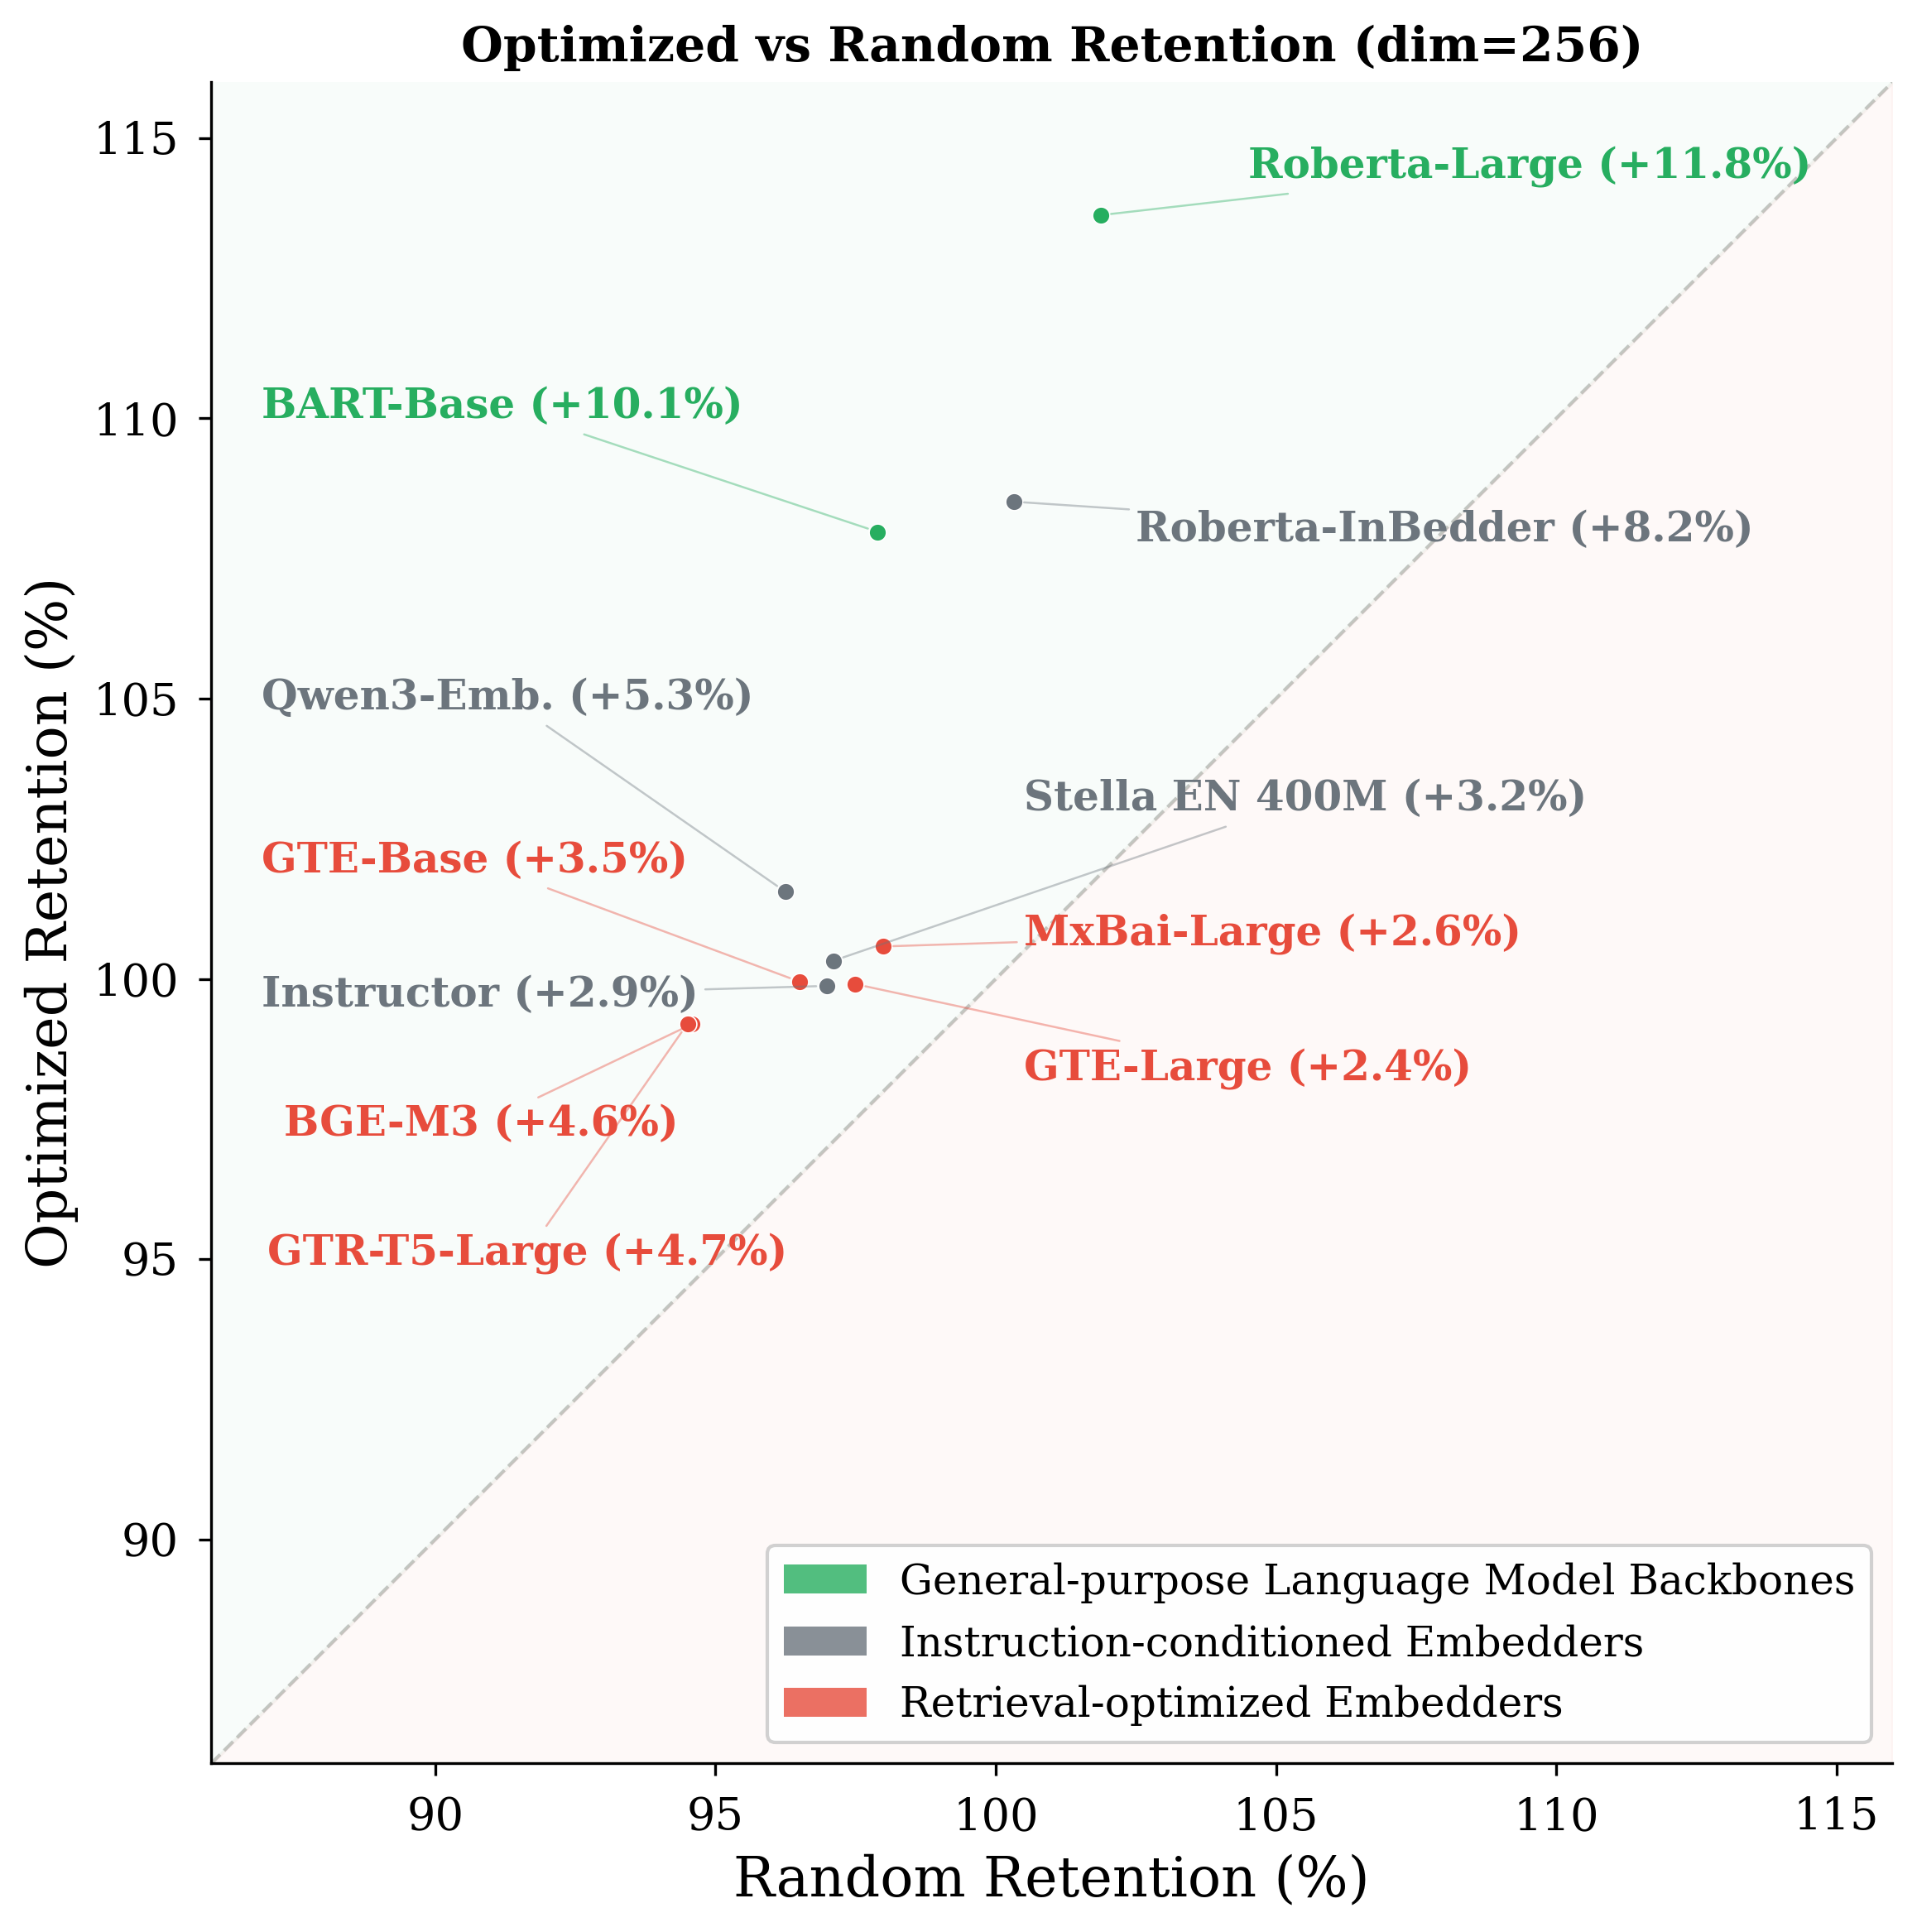
\includegraphics[width=\linewidth]{figures/fig_opt_vs_rnd_scatter.png}
    \caption{Optimized retention versus random retention. The dashed identity line marks parity. Green marks General-purpose Language Model Backbones, gray marks Instruction-conditioned Embedders, and red marks Retrieval-optimized Embedders.}
    \label{fig:opt_random_combined_2}
\end{figure}

\subsection{Evaluation Metric}

For each model-task-method combination, we compute the \textbf{retention ratio}:
\begin{equation}
R^{M,T}_k = \frac{S^{M,T}_k}{S^{M,T}_{D}} \times 100\%
\end{equation}
where $S^{M,T}_k$ is the MTEB main metric (e.g., accuracy, nDCG, Spearman $\rho$) of model $M$ on task $T$ using $k$ dimensions, and $S^{M,T}_D$ is the full-dimensional ($D$) baseline score. Values above 100\% mean that the pruned score exceeds the full-dimensional score under this instance. We report mean retention across tasks with 95\% bootstrap confidence intervals. Paired model and method comparisons are assessed using paired $t$-tests and Wilcoxon signed-rank tests, with Holm--Bonferroni correction applied within each test family.

\section{Experimental Results and Analysis}
\subsection{Finding 1: Random Is Strong, but Task-Aware Gains Vary by Training Paradigm and Compression Level}

\begin{figure*}[t]
    \centering
    
\includegraphics[width=0.95\linewidth]{figures/fig10_all_methods_comparison.png}
    \caption{Comparison of all five pruning methods at dim=256 for three representative models. Error bars show standard deviation across tasks. Random, Sequential, and Magnitude cluster together (96--101\%), while Anti-optimized drops to 86--89\%. The optimized upper bound sits only slightly above the cluster for GTE-Large and Stella, but farther above it for Roberta-InBedder. Magnitude results are only available for GTE-Large and Stella.}
    \label{fig:all_methods}
\end{figure*}

We first compare optimized and random selection across compression levels. Figure~\ref{fig:pruning_ratio_sweep} shows the retention ratio from a single retained dimension up to 75\% retention (768 of 1024 dimensions) for representative models.

\begin{table}[t]
    \centering
    \caption{Optimized vs.\ random at dim=256. $\Delta$: mean retention gap with 95\% bootstrap CI. $d$: Cohen's $d$. $p_{\text{holm}}$: Holm-Bonferroni corrected across 11 tests.}
    \label{tab:optimized_vs_random}
    \small
    \resizebox{\columnwidth}{!}{%
    \begin{tabular}{lcccc}
        \toprule
        Model & $\Delta$ & 95\% CI & $d$ & $p_{\text{holm}}$ \\
        \midrule
        \multicolumn{5}{l}{\textit{Retrieval-optimized Embedders}} \\
        GTR-T5-Large        & +4.69\% & [+2.91\%, +6.61\%] & 0.84 & $<$0.001 \\
        BGE-M3              & +4.61\% & [+3.17\%, +6.07\%] & 1.04 & $<$0.001 \\
        GTE-Base            & +3.49\% & [+2.15\%, +4.97\%] & 0.82 & $<$0.001 \\
        MxBai-Embed-Large   & +2.59\% & [+1.51\%, +3.83\%] & 0.83 & $<$0.001 \\
        GTE-Large           & +2.41\% & [+1.48\%, +3.40\%] & 0.83 & $<$0.001 \\
        \midrule
        \multicolumn{5}{l}{\textit{Instruction-conditioned Embedders}} \\
        Roberta-InBedder    & +8.19\% & [+5.96\%, +10.62\%] & 1.17 & $<$0.001 \\
        Qwen3-Embedding     & +5.30\% & [+3.54\%, +7.28\%]  & 1.00 & $<$0.001 \\
        Stella EN 400M      & +3.22\% & [+2.16\%, +4.44\%]  & 0.93 & $<$0.001 \\
        Instructor-Large    & +2.89\% & [+1.80\%, +4.06\%]  & 0.83 & $<$0.001 \\
        \midrule
        \multicolumn{5}{l}{\textit{General-purpose Language Model Backbones}} \\
        Roberta-Large       & +11.75\% & [+8.61\%, +15.53\%] & 1.16 & $<$0.001 \\
        BART-Base           & +10.08\% & [+6.30\%, +13.72\%] & 0.90 & $<$0.001 \\
        \bottomrule
    \end{tabular}%
    }
\end{table}

\paragraph{Optimization gains vary by training paradigm.}
The optimized selection strategy consistently outperforms random at dim=256 across the 11 models tested, but the gap varies systematically across the groups, as shown in Figure~\ref{fig:opt_random_combined_2} and Table~\ref{tab:optimized_vs_random}. Among the Retrieval-optimized Embedders, the gaps are the smallest ($+2.4\%$--$4.8\%$), with random selection retaining 95--98\% of full-dimension performance. Among the Instruction-conditioned Embedders except Roberta-InBedder, the gaps are also modest at $+2.9\%$--$5.3\%$, with random retention of 95--97\%. Table~\ref{tab:category_summary} breaks down the GTE-Large retention ratios by task category at dim=256. Appendix Table~\ref{tab:per_task_gte} reports the full per-task results for all 34 tasks. Note that the optimized method is an oracle that evaluates every chunk on the target task. The reported gap therefore serves as an upper bound on the gains that any practical task-aware method could hope to achieve. In contrast, Roberta-InBedder and General-purpose Language Model Backbones show larger optimized-random gaps ($+8.2\%$--$11.8\%$) that would materially affect downstream performance. Appendix~\ref{sec:Inbedder-mechanism} provides further analysis of how the training paradigm affects the optimized--random gap.

\begin{table}[t]
    \centering
    \caption{Mean retention (\%) by task category for GTE-Large at dim=256. Values are averaged across all tasks within each category.}
    \label{tab:category_summary}
    \resizebox{\columnwidth}{!}{
    \begin{tabular}{lccccc}
        \toprule
        Task Category & Random & Sequential & Magnitude & Optimized & Anti-optimized \\
        \midrule
        Classification & 97.3 & 97.8 & 96.9 & 101.4 & 84.2 \\
        Clustering & 95.1 & 95.0 & 95.4 & 99.4 & 81.5 \\
        Retrieval & 94.3 & 93.8 & 92.0 & 94.3 & 93.3 \\
        Reranking & 98.8 & 98.3 & 98.0 & 100.4 & 96.0 \\
        STS & 99.1 & 99.2 & 98.4 & 101.1 & 95.5 \\
        Pair Classification & 99.4 & 99.2 & 99.2 & 100.9 & 97.2 \\
        Summarization & 99.8 & 100.4 & 98.5 & 98.7 & 98.8 \\
        \bottomrule
    \end{tabular}
}
\end{table} 

\paragraph{Sequential and random remain close, while optimization gains scale with compression.}
Figure~\ref{fig:pruning_ratio_sweep} compares sequential and random selection across all tested retained dimensions, from 1 to 768 out of 1024. Their gap is consistently small and remains statistically insignificant throughout the pruning sweep. Appendix~\ref{sequential} provides more detailed statistics. In contrast, the optimized--random gap increases as compression becomes more severe. At the moderate 256-dimensional setting, the gap is only $+2.4$--$5.3\%$ for Retrieval-optimized Embedders and Instruction-conditioned Embedders other than Roberta-InBedder. At 64 retained dimensions, the gap widens to $+5.1$--$9.4\%$ for the same model group. This scaling pattern suggests that random selection is adequate under moderate compression, whereas task-aware methods become increasingly valuable as retained dimensionality shrinks. The transition point differs across model families, as detailed in Appendix~\ref{sec:gap_by_dim}.

\paragraph{Optimized gains generalize to held-out data.}
A natural concern is that the advantage of the optimized strategy may be inflated by evaluating on the same data used for ranking. We therefore conduct a train--test split validation in which chunks are ranked on the 70\% split and evaluated on the held-out 30\%. The optimized strategy remains above random on held-out data for all evaluated models and the same training-paradigm split persists: Retrieval-optimized Embedders and most Instruction-conditioned Embedders show smaller holdout gains (+1.52\%--2.70\%) than Roberta-InBedder and General-purpose Language Model Backbones (+4.02\%--5.15\%). This confirms that the oracle signal is not merely overfitting to the ranking data, while still leaving random selection highly competitive for Retrieval-optimized Embedders and most Instruction-conditioned Embedders. Full results are in Appendix~\ref{sec:train_test_split}.

\paragraph{Anti-optimized confirms dimensions carry information.}
Anti-optimized selection degrades performance to 84--91\% of baseline across the three models (Figure~\ref{fig:all_methods}). This shows that dimensions do carry task-relevant information. The key insight is that this information is spread so broadly that the specific subset chosen has minimal impact, as long as a sufficient number of dimensions are retained.

\subsection{Finding 2: Stronger Selection Strategies Struggle to Outperform Random}

Magnitude-based selection (keep the dimensions with the largest L2 norms of embedding weights) is perhaps the most natural zero-cost heuristic. If larger weights really marked more useful dimensions, this method should beat random selection. We test that intuition directly, and then ask whether stronger signals that use task embeddings, labels, or learned masks can do better. Together, these baselines test whether practical importance estimates can consistently improve over random without the full cost of optimized selection evaluation.

\paragraph{Magnitude performs equal to or worse than random.}
Magnitude-based pruning is much weaker than its intuitive appeal would suggest. Among Retrieval-optimized Embedders and most Instruction-conditioned Embedders, magnitude selection usually stays near Random ($-$1.7\%--+0.1\%). Roberta-InBedder and General-purpose Language Model Backbones suffer clearer degradation from Magnitude-based pruning. This pattern suggests that weight magnitude is a weak zero-cost heuristic rather than a practical replacement for random selection. Figure~\ref{fig:magnitude}(b--c) provide more detailed model-level and category-level breakdowns. Appendix~\ref{magnitude} further provides a more detailed analysis of why magnitude-based selection fails.

\paragraph{Stronger baselines also fail to outperform random.}
\label{sec:finding4}
\begin{table}[t]
    \centering
    \caption{Mean retention of gradient saliency, activation variance, and learned-mask selection on 8 representative tasks at 256 dimensions. Gradient and activation variance can be actively harmful for Roberta-InBedder and Roberta-Large.}
    \label{tab:strong_baselines}
    \small
    \resizebox{\columnwidth}{!}{%
    \begin{tabular}{lcccc}
        \toprule
        Model & Random & Gradient & Activation Variance & Mask \\
        \midrule
        \multicolumn{5}{l}{\textit{Retrieval-optimized Embedders}} \\
        GTE-Large & 99.5\% & 99.5\% & 99.7\% & 98.9\% \\
        BGE-M3 & 96.8\% & 97.1\% & 97.6\% & 96.4\% \\
        \midrule
        \multicolumn{5}{l}{\textit{Instruction-conditioned Embedders}} \\
        Stella EN 400M & 98.8\% & 99.3\% & 98.4\% & 98.3\% \\
        Roberta-InBedder & 100.1\% & 94.8\% & 93.3\% & 98.5\% \\
        \midrule
        \multicolumn{5}{l}{\textit{General-purpose Language Model Backbones}} \\
        Roberta-Large & 102.9\% & 93.4\% & 92.4\% & 102.0\% \\
        \bottomrule
    \end{tabular}%
    }
\end{table}

\begin{figure}[t]
    \centering
    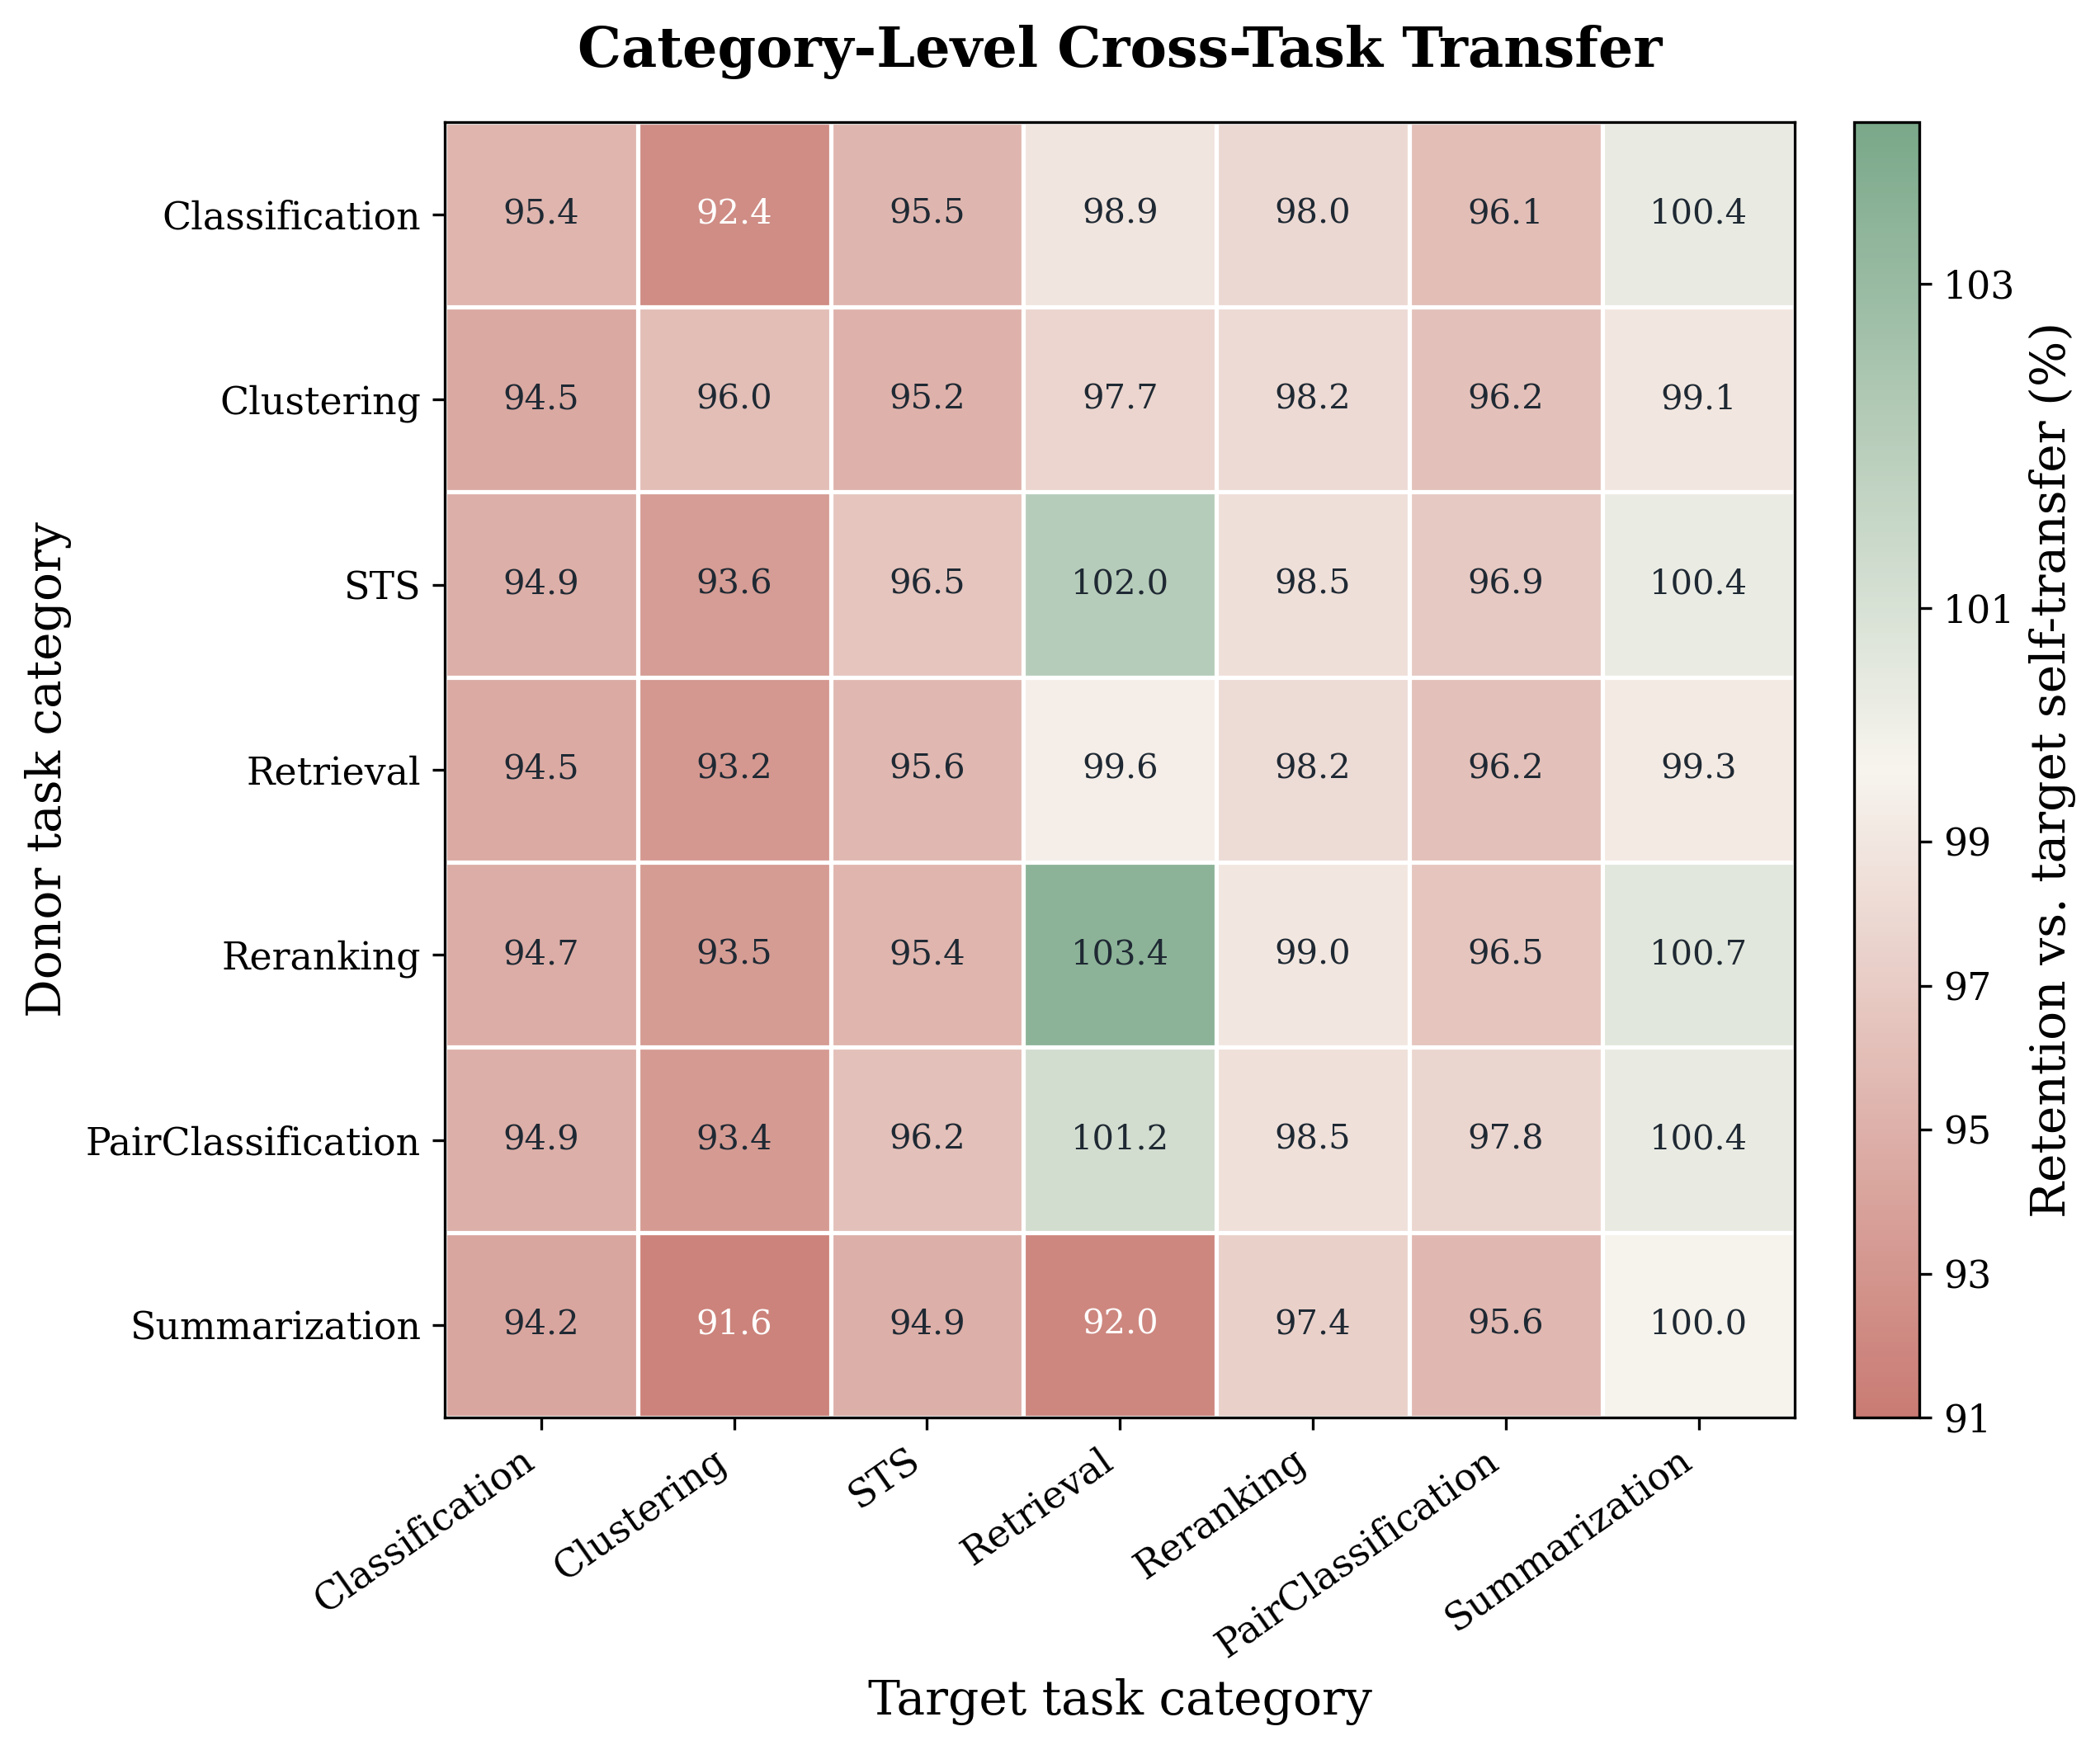
\includegraphics[width=0.78\linewidth]{figures/fig5_category_transfer.png}
    \caption{Mean category-to-category transfer retention (\%) at dim=256, averaged across 11 models. The matrix is strikingly uniform.}
    \label{fig:category_transfer}
\end{figure}

We test gradient-based importance, activation variance, and learned masks on 5 models (Table~\ref{tab:strong_baselines}). For Retrieval-optimized Embedders and Stella, gains are nearly zero ($-$0.5--+0.8\%). For Roberta-InBedder and Roberta-Large, gradient and activation-variance methods are \emph{harmful}: performance drops up to 10.5\%. Table~\ref{tab:pca_comparison} further shows that random selection is competitive with PCA and random projection under moderate compression. At $d=256$, all three methods retain at least 95.6\% performance across the tested models. The main difference appears under stronger compression: at $d=64$, random selection is much more stable on Roberta-InBedder and Roberta-Large, retaining 96.7--98.4\% where PCA falls to about 81\%. Therefore, random selection offers a simple deployment tradeoff. Appendix~\ref{sec:retrieval_cost} further reports the corresponding retrieval-system cost.

\begin{table}[t]
    \centering
    \caption{Random selection vs. projection-based compression, comparing random selection (RS), PCA, and random projection (RP) at 64 and 256 dimensions across representative models.}
    \label{tab:pca_comparison}
    \small
    \resizebox{\columnwidth}{!}{%
    \begin{tabular}{llccc}
        \toprule
        Model & Dim & PCA & RP & RS \\
        \midrule
        \multirow{2}{*}{GTE-Large}
            & 64  & 90.2\% & 92.9\% & 93.1\% \\
            & 256 & 98.0\% & 98.7\% & 99.0\% \\
        \multirow{2}{*}{BGE-M3}
            & 64  & 85.9\% & 87.2\% & 87.8\% \\
            & 256 & 95.8\% & 96.4\% & 96.1\% \\
        \multirow{2}{*}{Stella EN 400M}
            & 64  & 92.0\% & 93.9\% & 94.4\% \\
            & 256 & 98.5\% & 98.6\% & 98.9\% \\
        \multirow{2}{*}{Roberta-InBedder}
            & 64  & 80.8\% & 90.4\% & 96.7\% \\
            & 256 & 95.6\% & 98.4\% & 98.0\% \\
        \multirow{2}{*}{Roberta-Large}
            & 64  & 80.6\% & 91.2\% & 98.4\% \\
            & 256 & 99.9\% & 99.6\% & 100.2\% \\
        \bottomrule
    \end{tabular}%
    }
\end{table}

\subsection{Finding 3: Cross-Task Transfer Matches Random Selection}
\label{sec:finding3}

If dimension importance were highly task-specific, task-derived rankings should outperform random selection only when the source and target tasks match. We test this prediction via cross-task transfer, selecting dimensions by the source task's chunk ranking and evaluating them on the target task.

\paragraph{Transfer is nearly identical to random selection.}
Table~\ref{tab:cross_task_multidim} reports mean retention comparison for cross-task transfer and random selection, showing cross-task transfer barely improves over random. The all-pair gap is only +0.8\% at 256 dimensions and never exceeds +1.7\% across the 16--512 range. Appendix~\ref{sec:multidim_appendix} reports per-model and category-level breakdowns.

\paragraph{No category-level specialization.} Figure~\ref{fig:category_transfer} shows the mean transfer retention grouped by source and target task categories. The matrix is strikingly uniform, with no source category consistently providing better or worse rankings and no target category being particularly sensitive to the choice of source.

\begin{table}[t]
    \centering
    \caption{Pooled cross-task transfer vs.\ random selection across 11 models. Transfer remains close to random across all retained dimensions. ``All gap'' includes diagonal self-transfer. ``Off-diagonal gap'' excludes same-task source--target pairs. Per-model and category breakdowns are shown in Appendix~\ref{sec:multidim_appendix}.}
    \label{tab:cross_task_multidim}
    \small
    \resizebox{\columnwidth}{!}{%
    \begin{tabular}{lcccc}
        \toprule
        Retained Dims & Transfer & Random & All gap & Off-diagonal gap \\
        \midrule
        16 & 64.8\% & 63.8\% & +1.0\% & +0.7\% \\
        32 & 76.3\% & 75.3\% & +1.0\% & +0.7\% \\
        64 & 86.7\% & 85.6\% & +1.0\% & +0.8\% \\
        128 & 94.3\% & 93.4\% & +0.9\% & +0.7\% \\
        256 & 99.1\% & 98.3\% & +0.8\% & +0.7\% \\
        512 & 101.5\% & 99.8\% & +1.7\% & +1.6\% \\
        \bottomrule
    \end{tabular}%
    }
\end{table}

A striking aspect of these results is that disagreement over the importance rankings does not translate into disagreement in downstream retention. Appendix~\ref{paradox} examines this paradox in detail.

\begin{figure*}[!t]
    \centering
    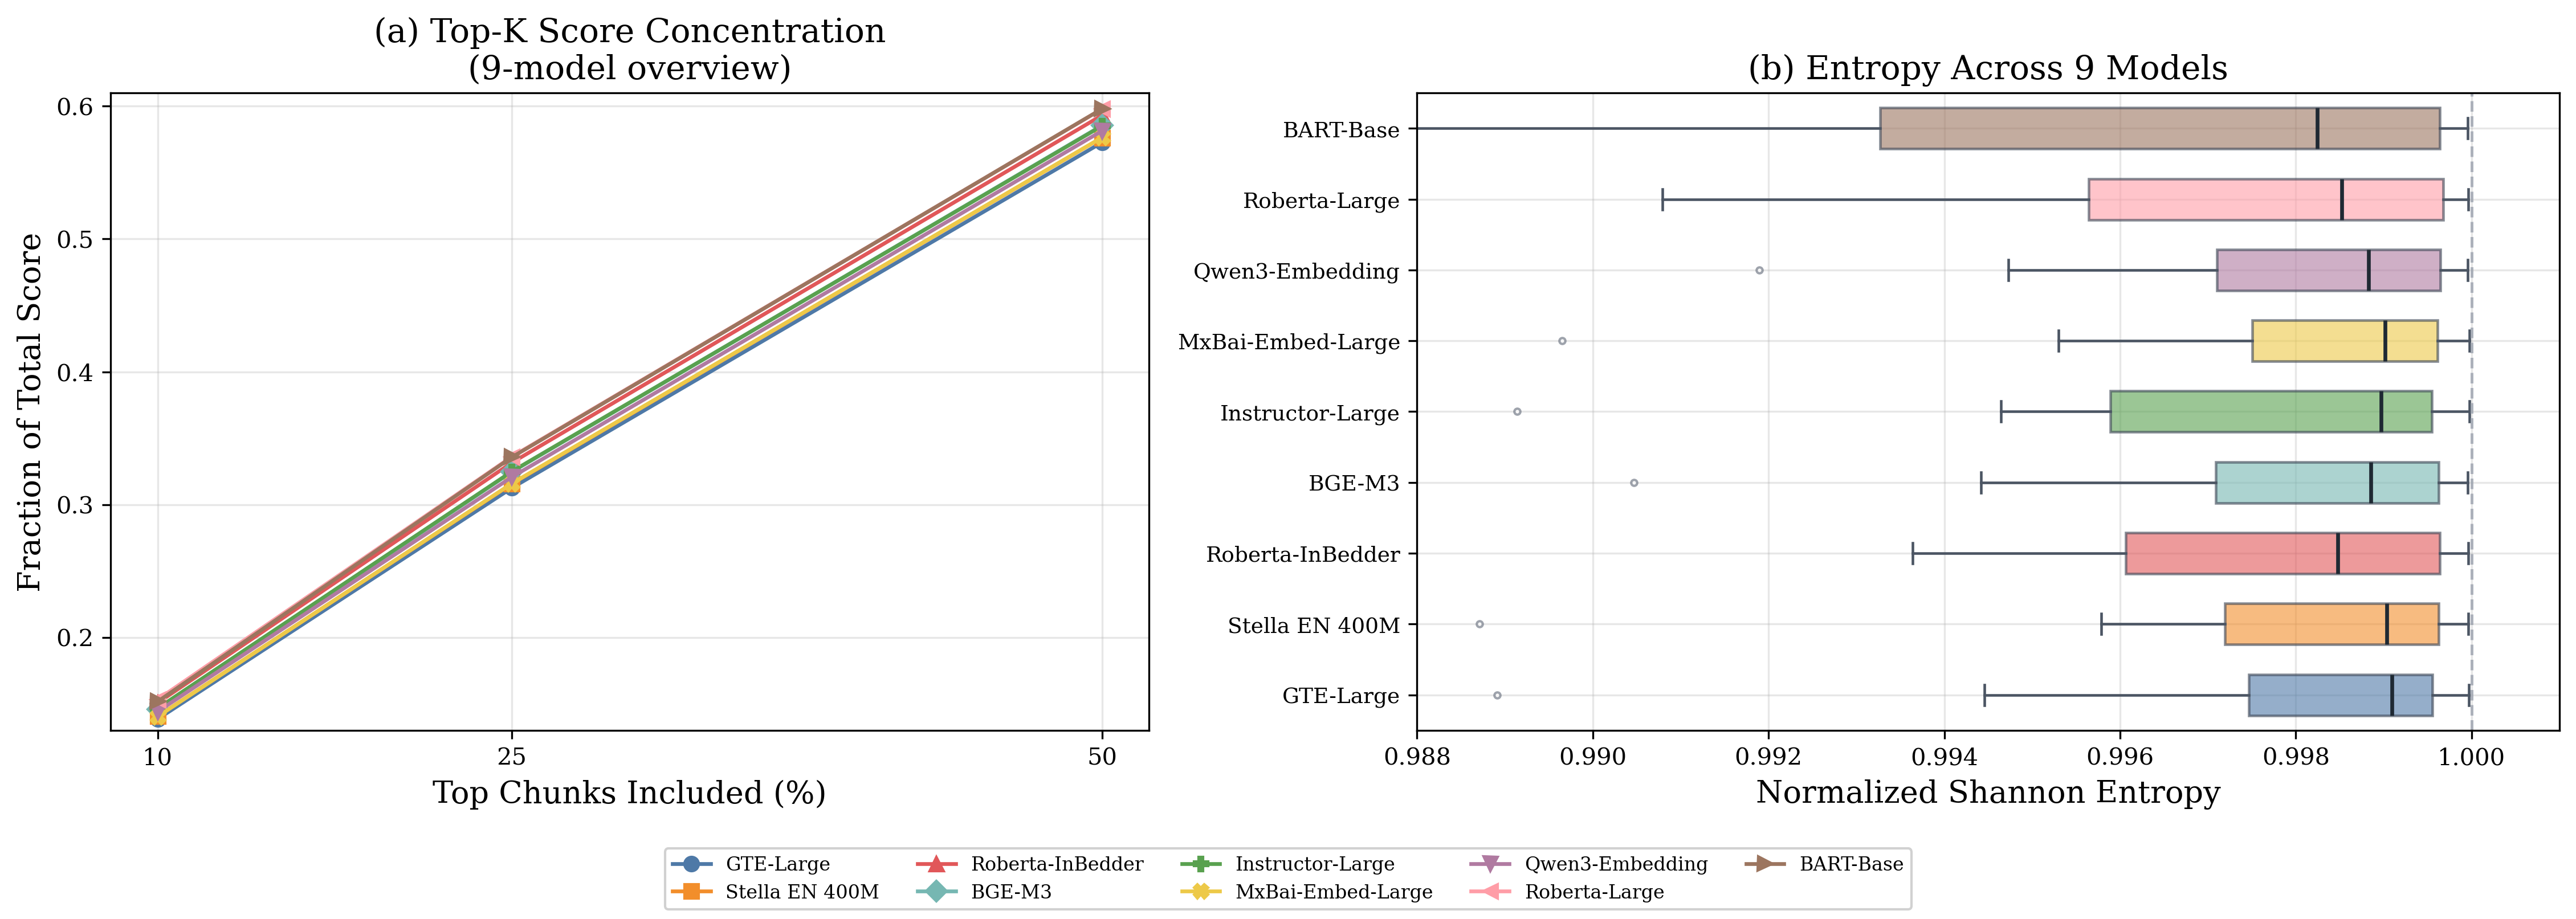
\includegraphics[width=0.95\linewidth]{figures/fig8_evidence_summary.png}
    \caption{(a) Top--k concentration curves for 9 models. The gradual, almost linear rise shows that importance is spread broadly across dimensions. (b) Boxplots of normalized Shannon entropy for the same 9 models. Model means stay close to the uniform upper bound (0.989--0.994), indicating remarkable consistency.}
    \label{fig:mechanism_summary}
\end{figure*}

\section{Mechanism: Universal Redundancy}

The findings above raise a question: why does random selection remain competitive with more informed selection strategies in many cases? Our evidence suggests that task-relevant information is distributed broadly across embedding dimensions. With no small subset dominating performance, nearly all sufficiently large subsets preserve most information.

\paragraph{Dimension importance is nearly uniform.}
To measure how evenly dimension importance is spread, we compute the normalized Shannon entropy of the chunk-level importance distribution. For each model-task pair, the importance of chunk $i$ is its task-specific evaluation score $S_i^T$ (from the optimized selection procedure in Section~\ref{sec:method}), and $p_i = S_i^T / \sum_j S_j^T$ is the normalized importance. We then compute:
\begin{equation}
H_{\text{norm}} = -\frac{1}{\log_2 N} \sum_{i=1}^{N} p_i \log_2 p_i
\end{equation}
where $N$ is the total number of chunks. $H_{\text{norm}} = 1$ means perfectly uniform importance. As shown in Figure~\ref{fig:mechanism_summary}(b), $H_{\text{norm}}=0.989-0.994$ across all models, indicating no small group of dimensions dominates the representation. Appendix~\ref{theoretical_perspective} provides a basis-dependence analysis. The same broad-distribution pattern appears under random orthogonal rotations, PCA, and whitening, suggesting that the result is not merely an artifact of the native coordinate basis. A complementary Shapley-based analysis shows a larger separation from standalone scoring, suggesting that chunk interactions contain additional structure, see Appendix~\ref{sec:loo}.

\paragraph{Importance accumulates gradually and linearly.}
Figure~\ref{fig:mechanism_summary}(a) shows the cumulative importance captured by the top-ranked chunks. If useful signal was concentrated in a few chunks, the curve would rise sharply. Instead, it rises gradually and linearly. Across the 9 models, the top 50\% of chunks capture only about 57--60\% of total importance, including General-purpose Language Model Backbones. This further suggests that that useful signal is spread broadly across dimensions, not concentrated in a few key dimensions.

\section{Discussion and Implications}

\paragraph{When does random work?}
Random selection already is a strong zero-cost baseline for Retrieval-optimized Embedders and most Instruction-conditioned Embedders. Magnitude-based pruning should be avoided despite its intuitive appeal, as it matches or underperforms random selection. Combined with the sequential $\approx$ random finding (Appendix~\ref{sequential}), none of the 3 task-agnostic selection strategies tested significantly outperforms the others. For embedding-specific models at moderate compression, as long as practitioners avoid deliberately selecting the worst dimensions, performance is robust to the choice of strategy. Appendix~\ref{sec:task_low_retention} and \ref{sec:random_variance} provide more detailed analyses of the risks associated with random selection.

\paragraph{When is random not enough?}
Two regimes demand task-aware selection: (1) General-purpose Language Model Backbones or specific Instruction-conditioned Embedders, where the optimized--random gap is substantially larger; (2) aggressive compression (dim $\leq$ 64), where random retention drops and variance increases sharply.
 
\paragraph{Implications for embedding model design.}
The universal redundancy we observe suggests that current embedding models are significantly overparameterized. A more promising design direction is therefore to train compact or dimension-adaptive representations from the start (e.g., Matryoshka-style training \citep{matryoshka2023}) rather than relying on post-hoc pruning. Importantly, our results motivate dimension-adaptive embeddings for predictable compression, since most off-the-shelf models lack a universally superior subset, while anti-optimized subsets remain clearly harmful. For a detailed comparison with Matryoshka Representation Learning, see Appendix~\ref{sec:matryoshka_comparison}.

\section{Conclusion}
We conduct a comprehensive investigation of dimension selection strategies for text embedding compression across 11 models and 34 MTEB tasks. Random dimension selection is a strong baseline for post-hoc compression of Retrieval-optimized Embedders and most Instruction-conditioned Embedders (+2.4--5.3\% at dim=256), but the gap is substantially larger for Roberta-InBedder and General-purpose Language Model Backbones (+8.2--11.8\%), suggesting that training paradigms shape how evenly information is distributed across dimensions.
The near-uniform importance we observe (entropy $= 0.989$--$0.994$) explains why random works. These findings establish a practical implication: for Retrieval-optimized Embedders and most Instruction-conditioned Embedders at moderate compression, random selection is the recommended default; for General-purpose Language Model Backbones or aggressive compression, task-aware selection provides meaningful gains. Future work should investigate whether these findings extend to multi-modal embeddings, and explore training-time interventions that preserve compression-friendly structure. Code and results will be released upon publication.

\section{Limitations}
The evaluation is based on a broad set of 34 MTEB tasks and 11 embedding models, but it does not cover every possible deployment setting or every task-aware compression method.

Our analysis focuses on off-the-shelf models without retraining. Models specifically trained for adaptive dimensionality may show different patterns. 

Our experiments study text embedding models. The same question may also be relevant for multi-modal embeddings, where representation geometry may differ. 

The observed association with training paradigm and compression level is empirical rather than theoretical. We do not provide a formal proof of this.

\bibliography{references,anthology}

\clearpage
\appendix

\section{Per-Task Results for GTE-Large}

Table~\ref{tab:per_task_gte} reports per-task retention at 256 dimensions (corresponding to a 75\% dimensionality reduction) for all 34 tasks in our benchmark on GTE-Large. Figure~\ref{fig:transfer_gte} shows the corresponding cross-task transfer matrix. For every source-target task pair, using the source task's importance ranking retains 93--100\% of the target task's performance. These detailed results complement the main-text averages by showing how retention varies across individual tasks for each pruning method.

\begin{table*}[h]
    \centering
    \caption{Per-task retention at dim=256 (75\% reduction) for all 34 tasks on GTE-Large. Random, Sequential, Optimized, and Anti-optimized use chunk-based selection (chunk size=2, top/bottom 128 of 512 chunks). Magnitude uses L2-norm ranking of embedding weights.}
    \label{tab:per_task_gte}
    \small
    \resizebox{\textwidth}{!}{
    \begin{tabular}{@{}p{5.8cm}ccccc@{}}
        \toprule
        Task & Random & Sequential & Magnitude & Optimized & Anti-optimized \\
        \midrule
        \multicolumn{6}{l}{\textit{Classification}} \\
        AmazonCounterfactualClassification & 95.8 & 97.3 & 93.6 & 105.6 & 70.0 \\
        AmazonReviewsClassification & 95.0 & 95.7 & 93.8 & 103.9 & 69.4 \\
        Banking77Classification & 99.3 & 99.4 & 99.4 & 100.0 & 98.1 \\
        EmotionClassification & 94.4 & 93.9 & 94.5 & 100.9 & 82.0 \\
        ImdbClassification & 99.3 & 100.3 & 98.7 & 100.9 & 77.5 \\
        MTOPDomainClassification & 99.0 & 99.0 & 99.0 & 99.9 & 95.5 \\
        MTOPIntentClassification & 97.8 & 97.5 & 97.2 & 99.2 & 94.7 \\
        MassiveIntentClassification & 98.0 & 98.6 & 98.2 & 99.5 & 96.7 \\
        MassiveScenarioClassification & 97.4 & 97.6 & 98.0 & 99.8 & 91.2 \\
        ToxicConversationsClassification & 96.9 & 98.5 & 96.4 & 105.0 & 66.6 \\
        TweetSentimentExtractionClassification & 97.9 & 98.0 & 97.0 & 101.2 & 84.8 \\
        \midrule
        \multicolumn{6}{l}{\textit{Clustering}} \\
        BiorxivClusteringS2S & 96.1 & 96.7 & 97.0 & 99.9 & 85.0 \\
        MedrxivClusteringS2S & 98.5 & 97.4 & 97.5 & 101.0 & 95.6 \\
        TwentyNewsgroupsClustering & 90.8 & 90.8 & 91.8 & 97.3 & 63.9 \\
        \midrule
        \multicolumn{6}{l}{\textit{Retrieval}} \\
        ArguAna & 96.7 & 96.4 & 97.6 & 96.7 & 96.7 \\
        CQADupstackEnglishRetrieval & 93.8 & 93.3 & 90.2 & 90.5 & 94.4 \\
        NFCorpus & 91.4 & 91.6 & 86.2 & 93.9 & 89.3 \\
        SCIDOCS & 92.9 & 92.6 & 90.5 & 93.0 & 89.7 \\
        SciFact & 96.9 & 95.1 & 95.7 & 97.6 & 96.3 \\
        \midrule
        \multicolumn{6}{l}{\textit{Reranking}} \\
        AskUbuntuDupQuestions & 99.2 & 97.7 & 97.8 & 102.2 & 96.6 \\
        SciDocsRR & 98.3 & 98.6 & 97.3 & 99.4 & 94.7 \\
        StackOverflowDupQuestions & 98.8 & 98.6 & 98.8 & 99.6 & 96.7 \\
        \midrule
        \multicolumn{6}{l}{\textit{STS}} \\
        BIOSSES & 98.8 & 99.1 & 98.9 & 105.1 & 94.0 \\
        SICK-R & 99.5 & 99.4 & 97.9 & 99.8 & 97.1 \\
        STS12 & 99.6 & 99.1 & 99.2 & 103.4 & 96.9 \\
        STS13 & 98.3 & 98.7 & 99.1 & 98.3 & 94.4 \\
        STS14 & 99.1 & 99.7 & 98.7 & 99.5 & 97.6 \\
        STS15 & 99.1 & 98.9 & 98.4 & 100.2 & 92.5 \\
        STS16 & 99.1 & 98.6 & 96.4 & 101.7 & 94.0 \\
        STSBenchmark & 99.2 & 99.7 & 98.2 & 100.4 & 97.6 \\
        \midrule
        \multicolumn{6}{l}{\textit{Pair Classification}} \\
        SprintDuplicateQuestions & 99.5 & 99.4 & 99.4 & 100.9 & 97.0 \\
        TwitterSemEval2015 & 99.3 & 98.9 & 98.9 & 101.7 & 96.4 \\
        TwitterURLCorpus & 99.4 & 99.3 & 99.2 & 100.0 & 98.3 \\
        \midrule
        \multicolumn{6}{l}{\textit{Summarization}} \\
        SummEval & 99.8 & 100.4 & 98.5 & 98.7 & 98.8 \\
        \midrule
        Mean & 97.5 & 97.5 & 96.7 & 99.9 & 90.6 \\
        \bottomrule
    \end{tabular}
    }
\end{table*}

\begin{figure*}[t]
    \centering
    
\includegraphics[width=0.95\linewidth]{figures/fig9_magnitude_comparison.png}
    \caption{(a) Spearman rank correlation between magnitude-based dimension ranking and task-specific importance ranking across five models. All mean correlations remain near zero. (b--c) Per-task magnitude vs.\ random retention. Points below the diagonal indicate tasks where random outperforms magnitude.}
    \label{fig:magnitude}
\end{figure*}

\section{Evaluation Coverage by Model}

Table~\ref{tab:model_list} summarizes which analyses are available for each of the 11 models in the study.

\begin{table*}[t]
    \centering
    \caption{Model coverage by experiment. ``Gap'' = optimized--random gap comparison and anti--optimized experiment.  “Magnitude” = magnitude pruning evaluation. ``Transfer'' = cross-task transfer analysis. ``Sweep'' = pruning-ratio sweep. ``Mechanism'' = entropy and uniformity analysis. ``Split'' = train/test split experiment. ``Tail'' = random-variance and tail-risk analysis. ``Stronger Baselines'' = stronger baselines including gradient, activation, PCA, learned selection. ``LOO'' = leave-one-out analysis. ``Cost'' = retrieval cost analysis. ``Chunk'' = chunk size sweep analysis.}
    \label{tab:model_list}
    \scriptsize
    \resizebox{\textwidth}{!}{%
    \begin{tabular}{lcccccccccccccccc}
        \toprule
        Model & Dims & Gap & Magnitude & Transfer & Sweep & Mechanism & Split & Tail & Strong Baselines & LOO & Cost & Chunk \\
        \midrule
        GTE-Large & 1024 & \checkmark & \checkmark & \checkmark & \checkmark & \checkmark & \checkmark & \checkmark & \checkmark & \checkmark & \checkmark & \checkmark\\
        Stella EN 400M & 1024 & \checkmark & \checkmark & \checkmark & \checkmark & \checkmark & \checkmark & \checkmark & \checkmark & \checkmark & \checkmark & \checkmark\\
        Roberta-Large & 1024 & \checkmark &  & \checkmark & \checkmark & \checkmark & \checkmark & \checkmark & \checkmark & \checkmark & \checkmark & \\
        BART-Base & 768 & \checkmark & \checkmark & \checkmark & \checkmark & \checkmark & \checkmark & \checkmark & & & & \\
        Roberta-InBedder & 1024 & \checkmark & \checkmark & \checkmark & \checkmark & \checkmark & \checkmark & \checkmark & \checkmark & \checkmark &  \checkmark & \checkmark \\
        BGE-M3 & 1024 & \checkmark & \checkmark & \checkmark & \checkmark & \checkmark & \checkmark & \checkmark  & \checkmark & \checkmark & \checkmark & \\
        Instructor-Large & 768 & \checkmark &  & \checkmark & \checkmark & \checkmark & \checkmark & \checkmark & & & & \\
        MxBai-Embed-Large & 1024 & \checkmark & \checkmark & \checkmark & \checkmark & \checkmark & \checkmark & \checkmark & & & & \\
        Qwen3-Embedding & 1024 & \checkmark & \checkmark & \checkmark & \checkmark & \checkmark & \checkmark & \checkmark & & & & & \\
        GTE-Base & 768 & \checkmark & \checkmark & \checkmark & & & & & & & & \checkmark\\
        GTR-T5-Large & 768 & \checkmark &  & \checkmark & & & & & & & & \checkmark\\
        \bottomrule
    \end{tabular}%
    }
\end{table*}

\begin{figure*}[t]
    \centering
    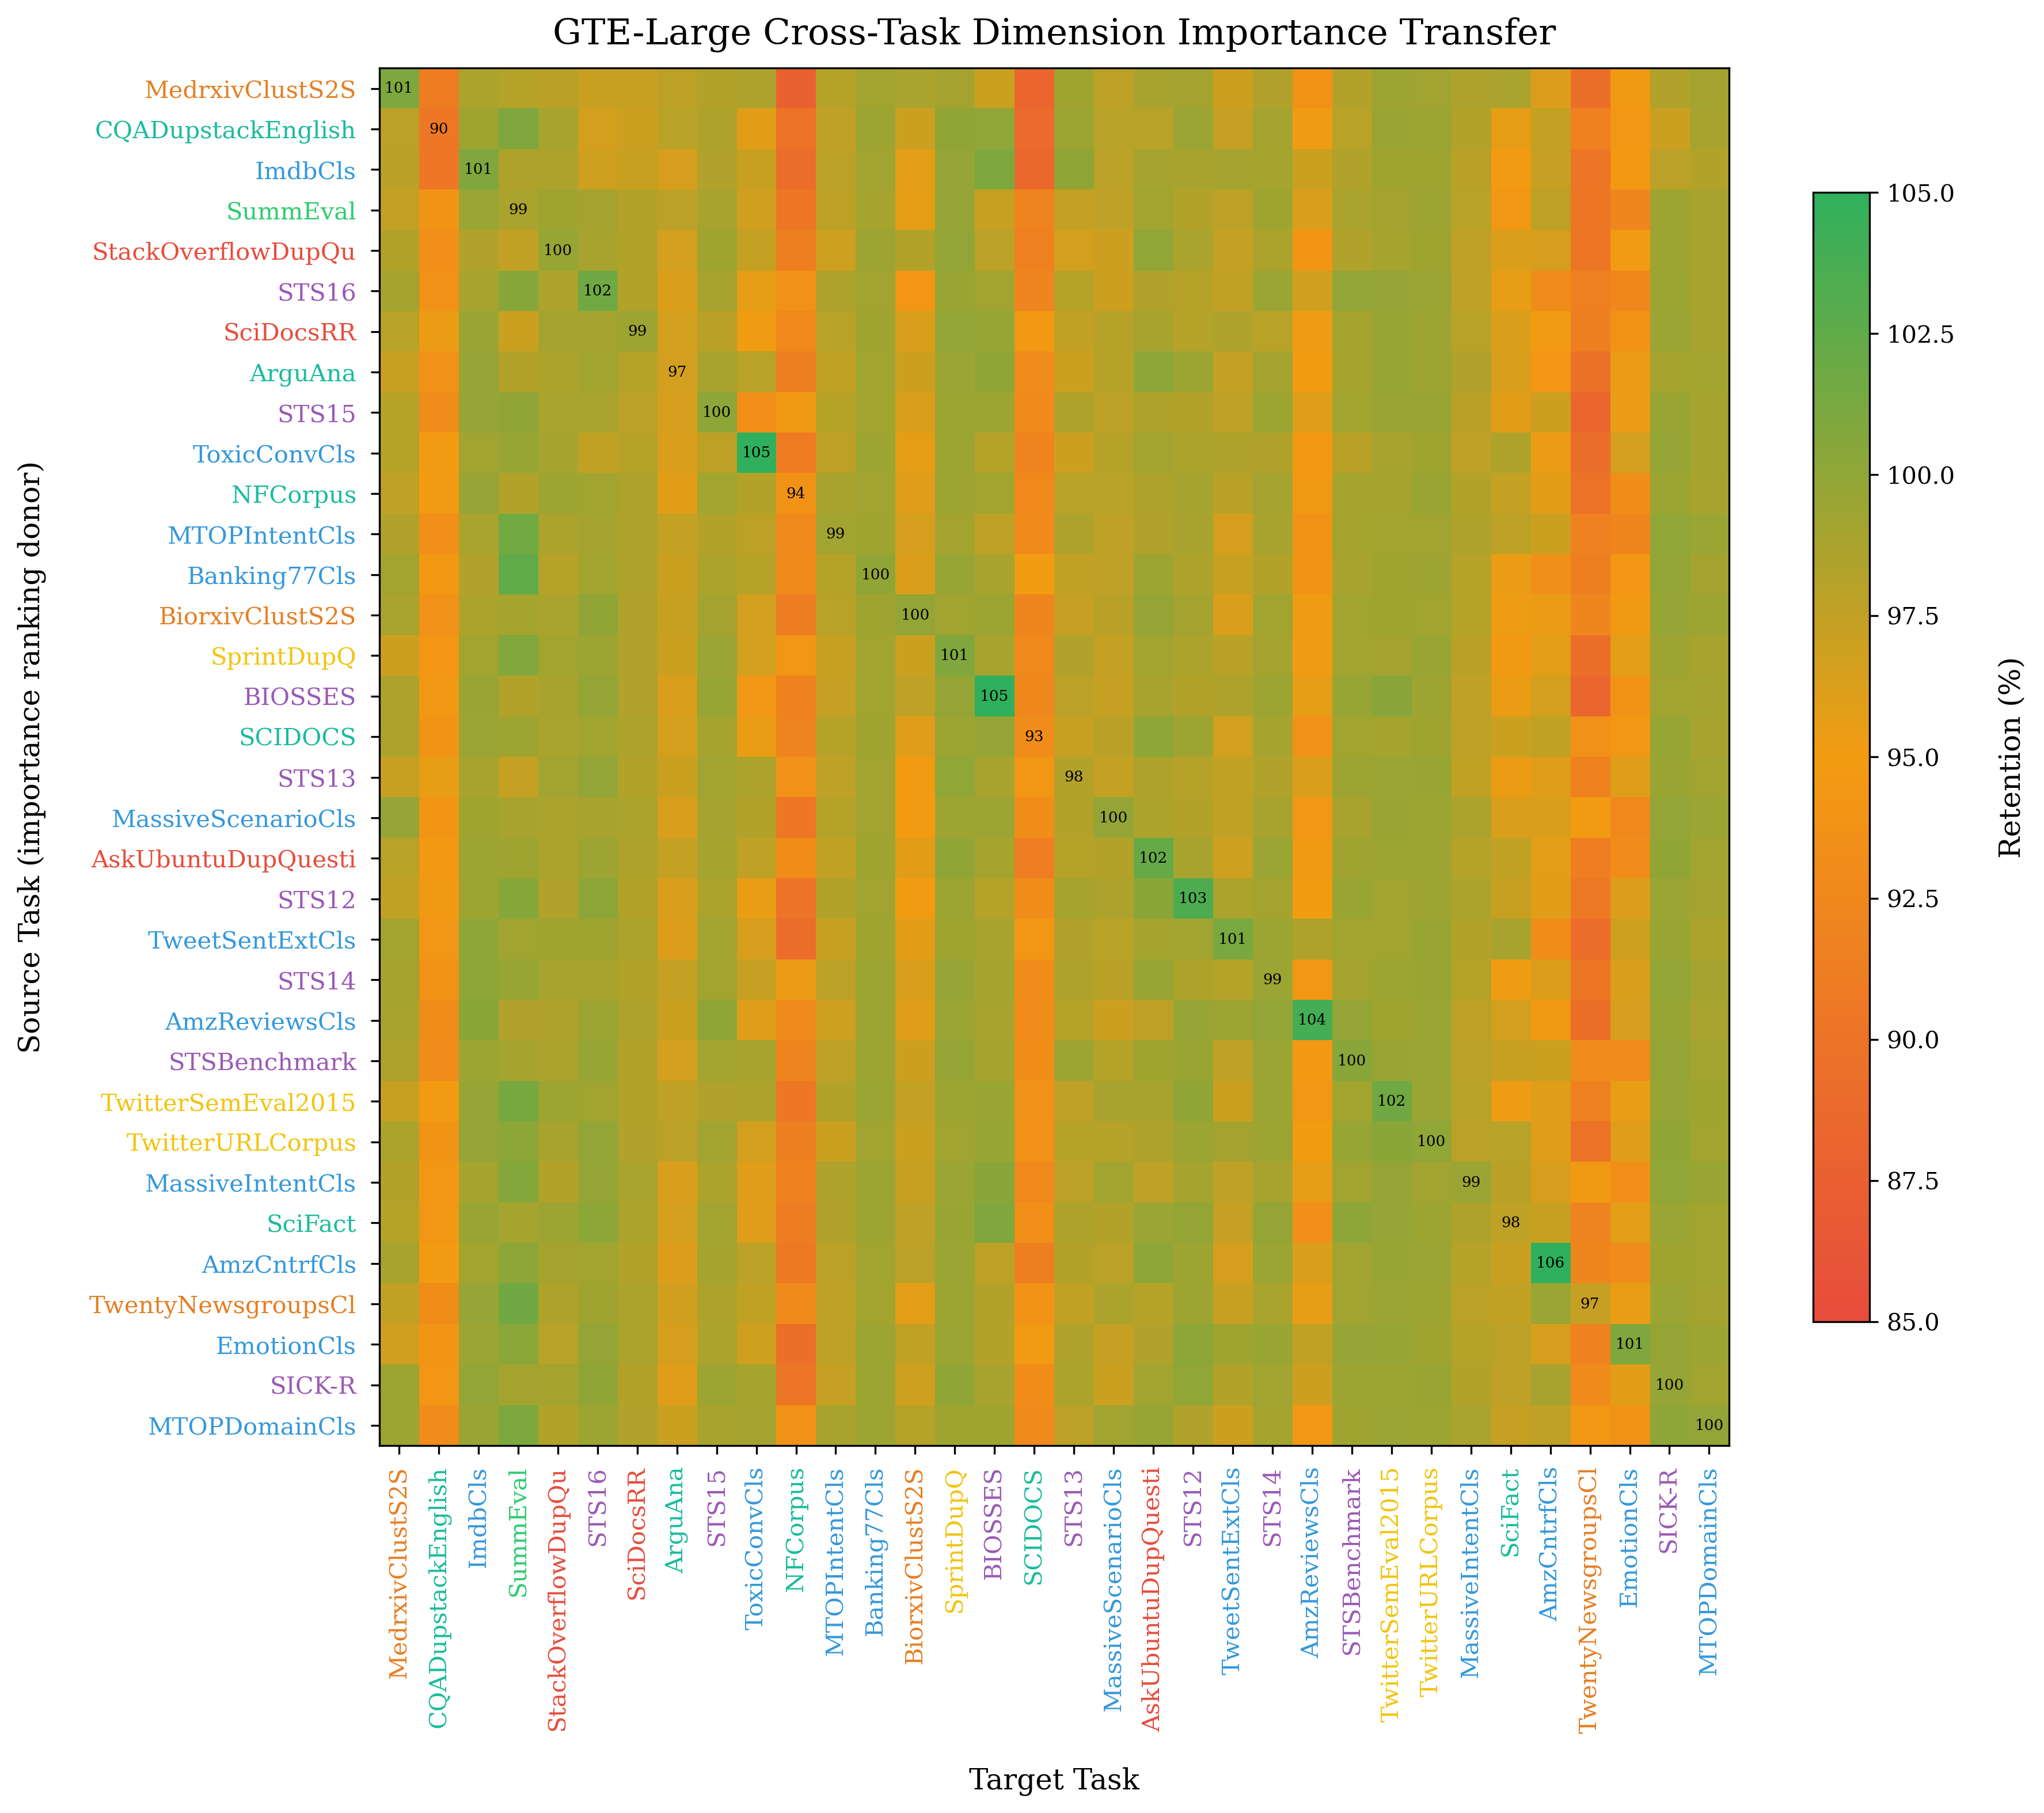
\includegraphics[width=0.95\linewidth]{figures/fig2_transfer_heatmap.png}
    \caption{Cross-task dimension importance transfer matrix for GTE-Large at dim=256. Each cell shows retention when using task $i$'s ranking to prune for task $j$.}
    \label{fig:transfer_gte}
\end{figure*}

\section{Chunk Size Sensitivity}
\label{sec:chunk_size}

We use chunk size $w = 2$ throughout the main experiments as a practical compromise between resolution and evaluation cost. For a typical 1024-dimensional model, evaluating single dimensions ($w = 1$) would require 1024 full task evaluations, while $w = 2$ cuts that to 512. Smaller chunks provide finer standalone scores but increase cost; larger chunks reduce cost but may hide within-chunk information. To verify that our conclusions are not sensitive to this choice, we sweep chunk sizes $w \in \{1, 2, 4, 8, 16, 32, 64\}$ on 5 models across 34 MTEB tasks.

\begin{table*}[h]
    \centering
    \caption{Optimized retention (\%) at dim=256 across chunk sizes averaged over 34 MTEB tasks. Random and Sequential baselines shown for reference. Bold marks the best chunk size per model.}
    \label{tab:chunk_sweep_full}
    \small
    \resizebox{\textwidth}{!} {
    \begin{tabular}{lccccccccc}
        \toprule
        & \multicolumn{7}{c}{Optimized retention at different chunk sizes $w$} & & \\
        \cmidrule(lr){2-8}
        Model & $w$=1 & $w$=2 & $w$=4 & $w$=8 & $w$=16 & $w$=32 & $w$=64 & Random & Seq \\
        \midrule
        \multicolumn{10}{l}{\textit{Retrieval-optimized Embedders}} \\
        GTE-Large & 99.9 & \textbf{99.9} & 99.6 & 99.4 & 99.4 & 99.2 & 98.9 & 97.5 & 97.5 \\
        GTE-Base & 99.9 & \textbf{100.1} & 99.8 & 99.1 & 98.8 & 98.3 & 98.2 & 96.6 & 96.6 \\
        GTR-T5-Large & \textbf{100.5} & 100.4 & 100.3 & 99.6 & 99.0 & 98.3 & 98.1 & 95.7 & 95.4 \\
        \midrule
        \multicolumn{10}{l}{\textit{Instruction-conditioned Embedders}} \\
        Roberta-InBedder & \textbf{108.7} & 108.5 & 107.4 & 107.0 & 108.1 & 108.0 & 107.4 & 100.3 & 101.3 \\
        Stella EN 400M & 100.1 & \textbf{100.3} & 100.2 & 100.2 & 99.8 & 99.2 & 99.0 & 97.1 & 97.1 \\
        \bottomrule
    \end{tabular}
    }
\end{table*}

Table~\ref{tab:chunk_sweep_full} shows the full results. Three findings emerge: (1) Optimized retention is nearly identical at $w = 1$ and $w = 2$ for all 5 models, indicating that the main optimized–random gaps are not an artifact of using paired dimensions. (2)~The optimized--random gap degrades gracefully as chunk size increases, and even $w = 64$ retains a positive gap for all models. (3)~The association between the optimized--random gap and training paradigm persists across chunk sizes. The gaps remain small for Retrieval-optimized Embedders and Stella EN 400M ($+1.4$--$4.8$\%), but are larger for Roberta-InBedder ($+6.7$--$8.4$\%). Thus, varying the chunk size does not change the main empirical conclusion: the value of task-aware pruning remains associated with training paradigm. These results support our choice of $w = 2$ for the main experiments.

\section{Optimized--Random Gap Across the Number of Retained Dimensions}
\label{sec:gap_by_dim}

Table~\ref{tab:optimized_random_gap_by_dim} reports how the optimized–random gap changes with the number of retained dimensions. The gap is consistently positive and grows as the number of retained dimensions shrinks, but the magnitude differs sharply by model family. At 256 dimensions, random is a strong baseline for Retrieval-optimized Embedders and most Instruction-conditioned Embedders. At 64, 32, and 16 dimensions, however, the task-aware advantage becomes larger even for those models. Roberta-InBedder and General-purpose Language Model Backbones show larger gaps throughout the sweep. Figure~\ref{fig:mechanism}(b) further shows the normalized gap between the optimized and worst chunk selections. The gap shrinks quickly as more chunks are retained, meaning that once the subset is large enough, the exact choice of chunks matters much less. The full sweep supports a more conditional claim: random selection is robust at moderate compression for embedding-specific models, whereas aggressive compression exposes more exploitable structure and increases the value of task-aware selection. 

\begin{table*}[!t]
    \centering
    \caption{Optimized--random gap across retained dimensions with chunk size $w=2$.}
    \label{tab:optimized_random_gap_by_dim}
    \small
    \resizebox{\textwidth}{!}{%
    \begin{tabular}{lcccccc}
        \toprule
        & \multicolumn{6}{c}{Retained dimensions} \\
        \cmidrule(lr){2-7}
        Model & $16$ & $32$ & $64$ & $128$ & $256$ & $512$ \\
        \midrule
        \multicolumn{7}{l}{\textit{Retrieval-optimized Embedders}} \\
        GTR-T5-Large      & +10.09\% & +9.69\% & +8.45\% & +6.88\% & +4.69\% & +2.35\% \\
        BGE-M3            & +11.06\% & +9.68\% & +8.10\% & +6.11\% & +4.61\% & +3.22\% \\
        GTE-Base          & +9.79\% & +8.44\% & +6.46\% & +4.73\% & +3.49\% & +1.82\% \\
        MxBai-Embed-Large & +9.66\% & +7.12\% & +5.11\% & +3.59\% & +2.59\% & +1.57\% \\
        GTE-Large         & +9.12\% & +7.31\% & +5.09\% & +3.31\% & +2.41\% & +1.72\% \\
        \midrule
        \multicolumn{7}{l}{\textit{Instruction-conditioned Embedders}} \\
        Roberta-InBedder  & +15.63\% & +14.33\% & +12.65\% & +10.92\% & +8.19\% & +6.18\% \\
        Qwen3-Embedding   & +13.90\% & +11.99\% & +9.44\% & +6.99\% & +5.30\% & +3.10\% \\
        Stella EN 400M    & +9.82\% & +8.15\% & +6.09\% & +4.68\% & +3.22\% & +2.03\% \\
        Instructor-Large  & +9.20\% & +7.97\% & +6.05\% & +4.30\% & +2.89\% & +1.44\% \\
        \midrule
        \multicolumn{7}{l}{\textit{General-purpose Language Model Backbones}} \\
        Roberta-Large     & +20.33\% & +19.09\% & +18.45\% & +15.01\% & +11.75\% & +11.73\% \\
        BART-Base         & +19.22\% & +16.81\% & +14.90\% & +13.87\% & +10.08\% & +3.73\% \\
        \bottomrule
    \end{tabular}%
    }
\end{table*}

\section{Sequential $\approx$ Random}
\label{sequential}
Sequential selection is essentially tied with random selection across the tested models (Figure~\ref{fig:pruning_ratio_sweep}). For GTE-Large, the sequential--random gap stays between $-0.76\%$ (at dim=4) and $+0.42\%$ (at dim=8). For Stella, it stays between $-0.69\%$ (at dim=2) and $+1.45\%$ (at dim=8). At the practically important dim=256 setting, the differences shrink to just $+0.03\%$ and $-0.02\%$, respectively.

The Cohen's $d$ effect size for sequential vs.\ random is $|d| < 0.02$, also confirming that the intrinsic ordering of dimensions carries no meaningful importance signal in GTE-Large and Stella. Roberta-InBedder shows only a small positive trend ($\Delta = +0.93\%$, Cohen's $d = 0.09$, $p = 0.070$), which is not statistically significant. This suggests that early dimensions do not have a consistent advantage over randomly selected dimensions in the evaluated models.

\section{Why does magnitude fail?}
\label{magnitude}

Magnitude measures a property of the \emph{embedding weights} process (how much each dimension is activated during encoding), but task performance depends on how activations are \emph{used downstream} (how they contribute to similarity computations), which may explain the failure of magnitude-based selection. Across the magnitude-based selection analysis conducted on 8 models, the magnitude--random gap is negative in six of seven task categories. The largest average penalty appears on retrieval (-7.65\%). This is notable because retrieval is precisely the task where dimension selection should matter most, requiring fine-grained similarity distinctions. Summarization is the only category with a positive mean gap. Figures~\ref{fig:magnitude}(b--c) visualize the model-level and category-level failures. 

Figure~\ref{fig:magnitude}(a) shows the Spearman rank correlation between magnitude-based dimension rankings and task-specific importance rankings. The mean correlations remain near zero for every tested model. In other words, a dimension's weight magnitude tells us almost nothing about how useful that dimension is for any downstream tasks. For GTE-Large, the top-128 chunks by magnitude share only 24 chunks (18.8\%) with the top-128 chunks by task importance (Jaccard index $= 0.10$). This near-random overlap ($\rho = -0.06$, $p = 0.15$) means that high-magnitude dimensions are essentially unrelated to task-relevant dimensions. The uniform importance distribution ensures that no weight-level property can reliably predict task-level importance, because magnitude picks dimensions that are prominent during encoding but not necessarily useful for the task. We note that this interpretation is speculative and would require gradient attribution analysis during training to validate, which we leave for future work.

\section{Full Multi-Dimension Cross-Task Transfer Results}
\label{sec:multidim_appendix}

Table~\ref{tab:multidim_appendix} extends the main body results (Table~\ref{tab:cross_task_multidim}) to all six retained dimensions and individual models. All values are mean retention across all source-target task pairs, including diagonal self-transfer.

\begin{table*}[t]
    \centering
    \caption{Cross-task transfer across six different retained dimensions for all 11 models with chunk size=2. Each cell is mean retention over all source-target pairs, including diagonal self-transfer. Random and Gap columns show random-selection retention and cross--task transfer--random gap at dim=256.}
    \label{tab:multidim_appendix}
    \small
    \resizebox{\textwidth}{!}{%
    \begin{tabular}{lcccccccc}
        \toprule
        Model & Transfer@16 & Transfer@32 & Transfer@64 & Transfer@128 & Transfer@256 & Transfer@512 & Random@256 & Gap@256 \\
        \midrule
        Roberta-Large & 67.0\% & 79.5\% & 93.5\% & 105.5\% & 114.0\% & 117.8\% & 111.5\% & +2.5\% \\
        Roberta-InBedder & 64.0\% & 75.9\% & 87.2\% & 96.2\% & 102.0\% & 104.8\% & 100.3\% & +1.7\% \\
        BART-Base & 64.4\% & 75.5\% & 85.5\% & 94.2\% & 100.1\% & 102.1\% & 97.9\% & +2.2\% \\
        GTE-Large & 67.8\% & 79.6\% & 88.8\% & 94.5\% & 97.6\% & 99.2\% & 97.5\% & +0.1\% \\
        Stella EN 400M & 67.5\% & 79.2\% & 88.5\% & 94.3\% & 97.5\% & 99.2\% & 97.1\% & +0.4\% \\
        MxBai-Embed-Large & 67.2\% & 78.8\% & 88.0\% & 93.9\% & 97.3\% & 99.1\% & 97.2\% & +0.1\% \\
        Instructor-Large & 64.4\% & 76.0\% & 86.1\% & 93.0\% & 97.0\% & 99.2\% & 97.0\% & +0.0\% \\
        Qwen3-Embedding & 64.9\% & 76.6\% & 86.2\% & 92.9\% & 96.8\% & 99.1\% & 95.5\% & +1.3\% \\
        GTE-Base & 63.1\% & 75.0\% & 85.5\% & 92.7\% & 96.8\% & 99.1\% & 96.6\% & +0.2\% \\
        GTR-T5-Large & 62.2\% & 72.9\% & 83.2\% & 91.0\% & 96.1\% & 98.9\% & 95.7\% & +0.4\% \\
        BGE-M3 & 60.3\% & 70.7\% & 81.0\% & 89.2\% & 94.9\% & 98.3\% & 94.6\% & +0.3\% \\
        \bottomrule
    \end{tabular}%
    }
\end{table*}

\section{The Paradox: Zero Correlation, High Retention}
\label{paradox}
We begin with the central paradox in our cross-task transfer results: chunk importance rankings differ almost completely across tasks, yet rankings derived from one task still transfer well to other tasks. To quantify the degree of cross-task disagreement, we compute, for each model, the Spearman correlation between the source-task and target-task standalone chunk-score vectors over the same N chunks. These correlations are essentially zero: the Spearman rank correlation between any two tasks’ dimension-importance rankings is $\rho \approx 0.001$. Despite this near-total lack of rank agreement, cross-task transfer still consistently outperforms random selection, as shown in Table~\ref{tab:cross_task_multidim}. Figure~\ref{fig:transfer_paradox} visualizes this contrast.

One possible resolution lies in low subset sensitivity. When many subsets produce similar retention, rankings can have near-zero correlation while still yielding similar downstream performance (Appendix~\ref{theoretical_perspective}). When importance is nearly uniform ($H_{\text{norm}} \to 1$), performance varies little across different chunk selections. If each chunk captures approximately $1/N$ of total importance, then any $k$-chunk selection should capture approximately $k/N$ of full-dimension importance, with variance proportional to $(1 - H_{\text{norm}})$. At $H_{\text{norm}} = 0.991$, that variance is very small. This explains why the cross-task transfer and random selection yield similar retention.

The near-zero ranking correlation is also consistent with this mechanism. When importance is almost uniform, tiny perturbations can change the order a lot without significantly changing the quality of the selected subset. To validate this empirically, we note that random selection (which uses no importance information at all) already retains about 95--98\% of full-dimension performance for Retrieval-optimized Embedders and for Instruction-conditioned Embedders except Roberta-InBedder. Since random selection achieves retention comparable to optimized selection, the specific ranking used for cross-task transfer is largely immaterial, making any reasonable selection achieve similar results, which is precisely what the transfer data shows.

\begin{figure*}[t]
    \centering
    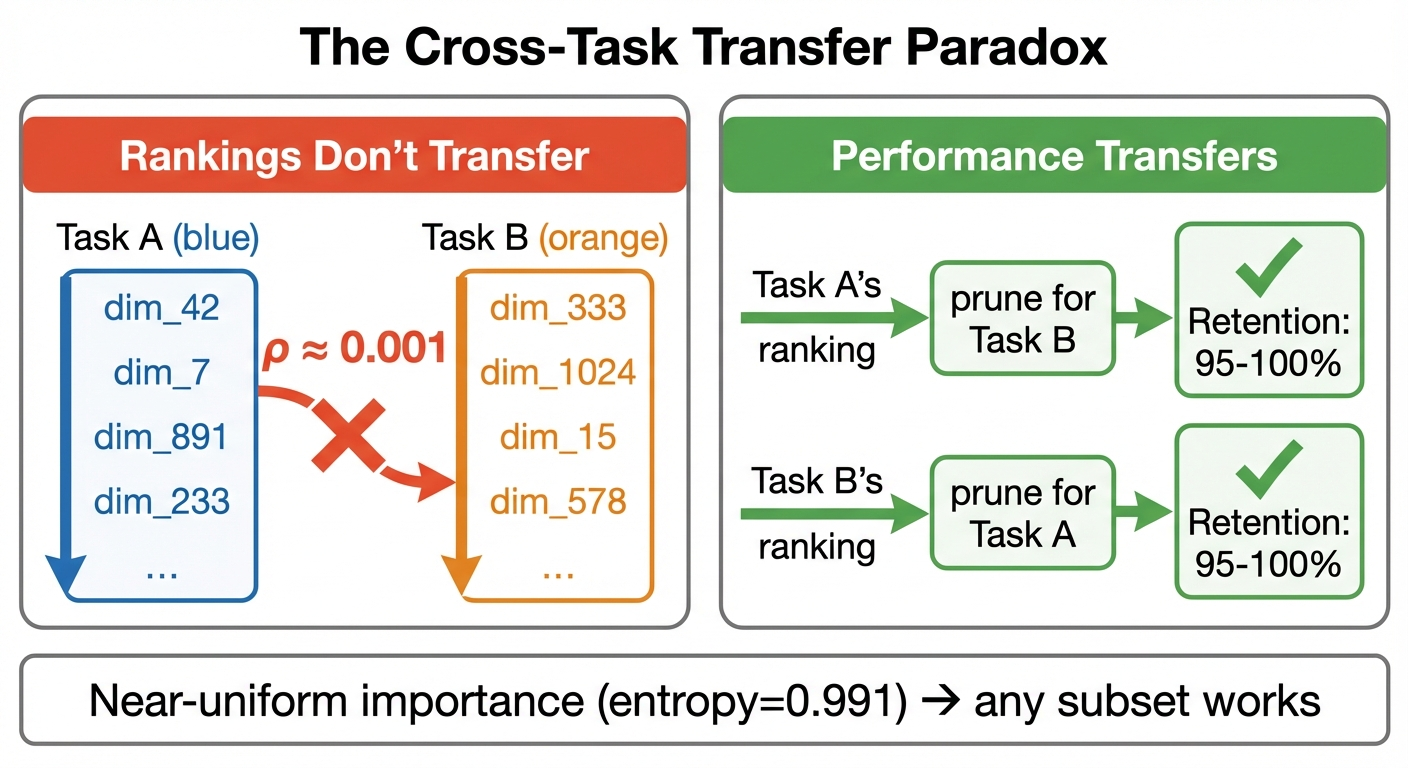
\includegraphics[width=0.95\linewidth]{figures/fig_transfer_paradox.png}
    \caption{The cross-task transfer paradox. Left: two tasks produce entirely different dimension importance rankings ($\rho \approx 0.001$). Right: despite this disagreement, using either task's ranking to prune for the other retains 91--100\% of performance. The resolution lies in near-uniform importance ($H_{\text{norm}} = 0.991$), indicating that nearly all sufficiently large subsets of dimensions preserve most information.}
    \label{fig:transfer_paradox}
\end{figure*}

\begin{figure*}[t]
    \centering
    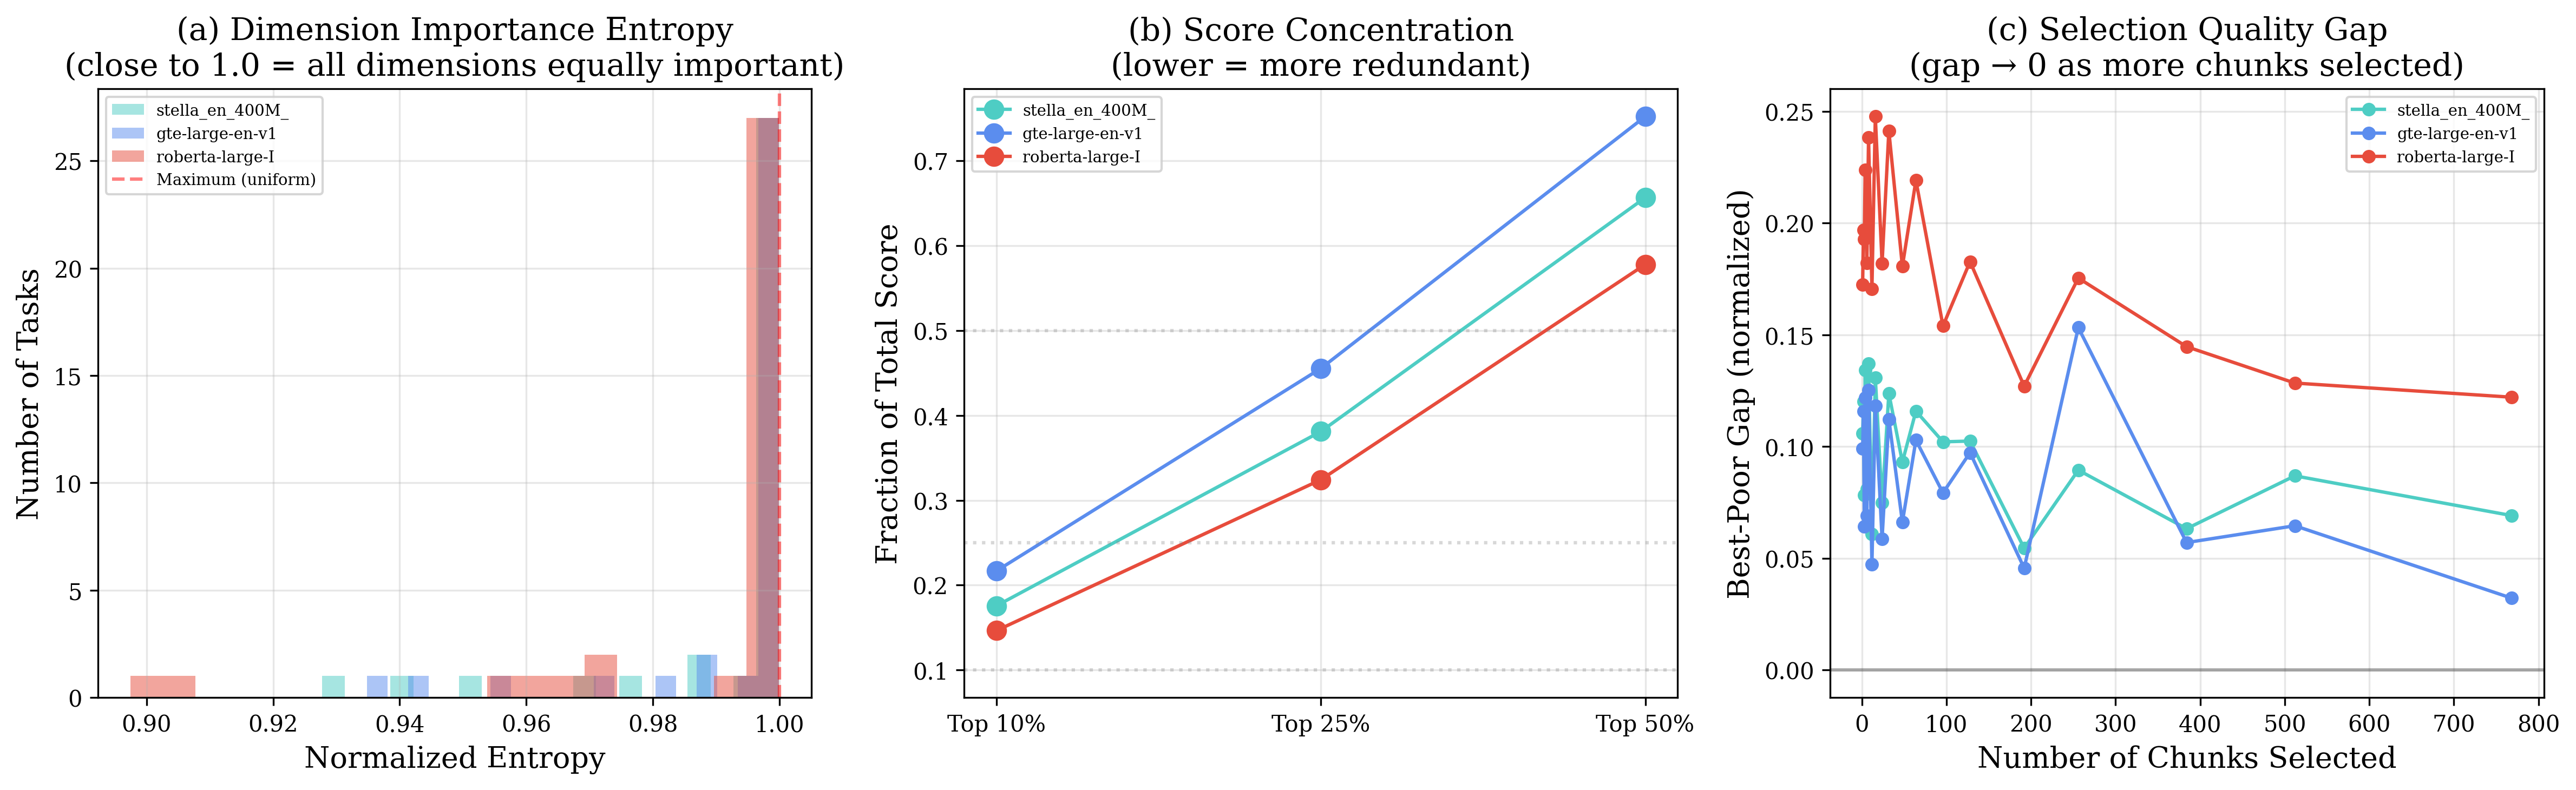
\includegraphics[width=0.95\linewidth]{figures/fig7_redundancy_mechanism.png}
    \caption{Representative views of the redundancy mechanism for the three focal models. (a) Histograms of per-task normalized entropy. Values near 1.0 indicate near-uniform importance. (b) Normalized optimized--worst selection gap as the number of selected chunks increases.}
    \label{fig:mechanism}
\end{figure*}

\section{Short Answer-Conditioned Supervision Is Associated with Greater Dimension Structure}
\label{sec:Inbedder-mechanism}

Our interpretation predicts that models trained on narrower data distributions should show less uniform importance. If diverse training spreads information evenly across dimensions, then narrower supervision should do so less effectively. We test that prediction with Roberta-InBedder, a model fine-tuned on abstractive question answering data whose target answers average only 2.89 tokens. Since the targets are typically extremely short, this supervision signal is substantially narrower than that of models trained on diverse contrastive pairs. As predicted, Roberta-InBedder exhibits one of the largest optimized-random gap (+8.19\% vs.\ +2.41\%--+5.30\% for Retrieval-optimized Embedders and other Instruction-conditioned Embedders, Table~\ref{tab:optimized_vs_random}), consistent with this narrower training signal being associated with slightly more dimension structure.

\paragraph{Characteristics of the exception.}
To understand why Roberta-InBedder differs, we compare its dimension importance distribution with one Retrieval-Optimized Embedder (GTE-Large) and one Instruction-Conditioned Embedder (Stella) (Table~\ref{tab:inbedder_mechanism}, Figure~\ref{fig:mechanism}). Its Gini coefficient is 0.124 vs.\ 0.101--0.107 for GTE-Large and Stella, its chunk-importance coefficient of variation is 0.242 vs.\ 0.186--0.195. Its normalized entropy is 0.990 vs.\ 0.993--0.994. While these absolute differences are small, the relative differences are consistent: Roberta-InBedder's importance distribution is measurably less uniform. Table~\ref{tab:inbedder_mechanism} also demonstrates that General-purpose Language Model Backbones show even lower entropy and higher Gini, confirming that training paradigm influences dimension structure.

\paragraph{Mechanism: short answer-conditioned supervision reduces uniformity.}
Roberta-InBedder shows consistently higher concentration of importance across all metrics than Retrieval-optimized Embedders and other Instruction-conditioned Embedders. A plausible interpretation is that two linked aspects of Roberta-InBedder's training matter here. Unlike embedding models trained on diverse data, Roberta-InBedder is fine-tuned on abstractive QA tasks, and the answer targets are extremely short on average (2.89 tokens). This combination may concentrate supervision on a narrower set of representation features, making some dimensions more aligned with the latent answer signal while others carry more task-irrelevant noise. 

\begin{table*}[!t]
    \centering
    \caption{Dimension importance distribution across five representative models. Cross-task retention is mean transfer retention at dim=256, chunk size=2.}
    \label{tab:inbedder_mechanism}
    \small
    \resizebox{\textwidth}{!}{%
    \begin{tabular}{lccccc}
        \toprule
        Metric & GTE-Large & Stella EN 400M & Roberta-InBedder & BART-Base & Roberta-Large \\
        \midrule
        Normalized entropy & 0.994 & 0.993 & 0.990 & 0.989 & 0.989 \\
        Gini coefficient & 0.101 & 0.107 & 0.124 & 0.130 & 0.131 \\
        Chunk importance CV & 0.186 & 0.195 & 0.242 & 0.252 & 0.255 \\
        Top-50\% concentration & 0.573 & 0.576 & 0.593 & 0.598 & 0.598 \\
        \midrule
        Optimized--random gap & +2.41\% & +3.22\% & +8.19\% & +10.08\% & +11.75\% \\
        \bottomrule
    \end{tabular}%
    }
\end{table*}

\begin{figure*}[t]
    \centering
    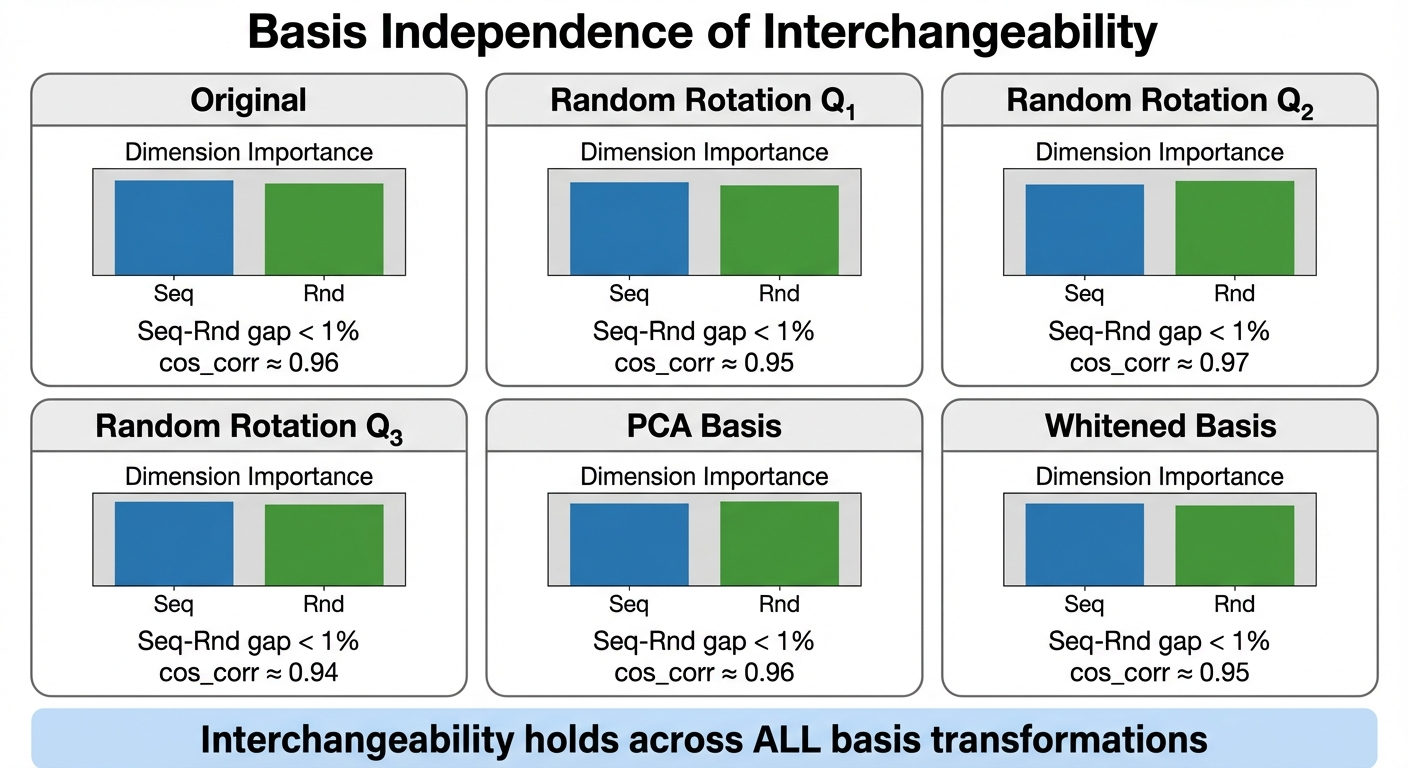
\includegraphics[width=0.95\linewidth]{figures/fig_basis_independence.png}
    \caption{Basis-dependence analysis of random selection. We apply six basis transformations to the embedding space (original, three random orthogonal rotations, PCA, and whitening) and measure the sequential--random gap and cosine--correlation preservation after pruning. In every basis, the gap stays below 1\% and cosine correlation exceeds 0.94, suggesting that the broad distribution of task-relevant information is not merely an artifact of one coordinate system.}
    \label{fig:basis_independence}
\end{figure*}

\paragraph{Pruning as implicit regularization.}
For Roberta-InBedder, pruning actually \emph{improves} performance on many tasks at dim=256. This is consistent with the well-established phenomenon in deep learning where removing parameters can act as implicit regularization \citep{han2015pruning,lottery-ticket}, reducing overfitting by eliminating dimensions that encode task-irrelevant noise. The higher importance variance in Roberta-InBedder (CV $= 0.242$ vs.\ $0.186$--$0.195$ for Retrieval-optimized Embedders and other Instruction-conditioned Embedders) means that optimized selection can better separate useful from noisy dimensions. This provides a practical diagnostic in that if a model shows large gaps between optimized and random selection, it may be overparameterized for its intended use case, and pruning could serve as a simple regularization strategy.

\section{Theoretical perspective: near-uniform importance as a design consequence}
\label{theoretical_perspective}
Our findings align with literature on intrinsic dimensionality \citep{li2018measuring,alemohammad2023intrinsic}, which shows that high-dimensional neural representations live on low-dimensional manifolds. We extend that perspective by arguing that the \emph{importance distribution across dimensions} is approximately uniform for models trained on broad, diverse contrastive data. This uniformity is unlikely to be accidental, since contrastive learning objectives encourage all dimensions to contribute to the similarity signal and any dimension that consistently carries useful gradients will be reinforced during training. The result is a uniformly distributed representation in which no dimension dominates.

The above intuition can be formalized as follows. Under a contrastive loss $\mathcal{L} = -\log[\exp(\mathbf{z}_i \cdot \mathbf{z}_j) / \sum_{k} \exp(\mathbf{z}_i \cdot \mathbf{z}_k)]$ where $\mathbf{z}_i$ is the representation of anchor $i$, $\mathbf{z}_j$ is the positive, and $\mathbf{z}_k$ ranges over all positives and negatives in the batch, each dimension $d$ contributes additively to the dot product. When the training data is broad and diverse, no single dimension can specialize too strongly without hurting performance elsewhere, so the contributions tend to balance out. Roberta-InBedder exception fits this picture in that its non-contrastive, answer-conditioned fine-tuning on very short QA answers is associated with a less even importance distribution and a larger task-aware advantage. Taken together, this reasoning suggests a clear prediction for future work: models trained with less diverse supervision should display less uniform importance distributions and, as a result, larger optimized–random gaps. A rigorous test of this prediction would require controlling for confounding factors by holding architecture and data fixed while varying the training objective, or by comparing matched model pairs that share the same embedding head and normalization. We leave this controlled investigation to future work.

A natural concern is that the small sequential-random gap might be an artifact of the native coordinate system in which the embedding dimensions are defined. To test that, we repeat the pruning analysis after several basis transformations, including random orthogonal rotations, PCA, and whitening. The sequential--random gap stays below 1\% in every basis (Figure~\ref{fig:basis_independence}). This suggests that the observed robustness of random selection is not merely a quirk of the native coordinate basis.

\section{Comparison with Matryoshka Representation Learning}
\label{sec:matryoshka_comparison}
Our findings provide an empirical lower bound on the value of learned dimension adaptation. \citet{matryoshka2023} show that MRL-trained models can achieve up to 14$\times$ embedding compression with only minor accuracy loss on classification and retrieval, but that benefit comes from special training with an adaptive loss. By contrast, our post-hoc first-$k$ truncation experiments show that simply taking the first 256 dimensions does not recover that property: sequential truncation remains essentially indistinguishable from random ($|d| < 0.02$). Importantly, Stella EN 400M stays near parity despite being MRL-trained, which suggests that once the representation is projected through its linear output head, naive prefix truncation no longer reveals a universally privileged prefix. A direct numerical comparison between MRL-trained and standard models on the same MTEB tasks would require re-implementing MRL training, which is beyond our current budget, so we leave that comparison to future work.

\section{Task-Level Low-Retention Outcomes}
\label{sec:task_low_retention}

The main text reports mean retention to compare various MTEB tasks on a common scale. However, a high mean may sometimes hide task-level failures. Therefore, table~\ref{tab:low_retention_random} reports low-retention summaries at dim=256. P25, P10, and P5 describe progressively lower parts of the task distribution, while the worst-task column identifies where each model is most sensitive.


\begin{table*}[t]
    \centering
    \caption{Random low-retention summaries at dim=256. P25, P10, and P5 are task-level percentiles. Worst task reports the lowest-retention task and its retention.}
    \label{tab:low_retention_random}
    \scriptsize
    \resizebox{\textwidth}{!}{%
    \begin{tabular}{lrrrrlrr}
        \toprule
        Model & Mean & P25 & P10 & P5 & Worst task & $<90$ & $>100$ \\
        \midrule
        \multicolumn{8}{l}{\textit{Retrieval-optimized Embedders}} \\
        GTR-T5-Large & 95.7\% & 92.6\% & 90.3\% & 89.3\% & SCIDOCS (88.4\%) & 3 & 1 \\
        BGE-M3 & 94.6\% & 91.9\% & 86.5\% & 84.0\% & SCIDOCS (80.2\%) & 7 & 0 \\
        GTE-Base & 96.6\% & 94.4\% & 93.1\% & 92.5\% & MTOPIntentClassification (91.2\%) & 0 & 0 \\
        MxBai-Embed-Large & 97.2\% & 96.1\% & 93.4\% & 92.7\% & NFCorpus (91.1\%) & 0 & 0 \\
        GTE-Large & 97.5\% & 96.8\% & 94.0\% & 92.4\% & TwentyNewsgroupsClustering (90.8\%) & 0 & 0 \\
        \midrule
        \multicolumn{8}{l}{\textit{Instruction-conditioned Embedders}} \\
        Roberta-InBedder & 100.3\% & 96.3\% & 94.2\% & 93.3\% & TwentyNewsgroupsClustering (91.4\%) & 0 & 11 \\
        Qwen3-Embedding & 95.5\% & 92.6\% & 90.6\% & 88.8\% & NFCorpus (83.6\%) & 3 & 0 \\
        Stella EN 400M & 97.1\% & 95.7\% & 93.0\% & 92.2\% & NFCorpus (89.8\%) & 1 & 1 \\
        Instructor-Large & 97.0\% & 95.8\% & 93.6\% & 91.9\% & NFCorpus (89.0\%) & 1 & 1 \\
        \midrule
        \multicolumn{8}{l}{\textit{General-purpose Language Model Backbones}} \\
        Roberta-Large & 111.5\% & 96.1\% & 90.8\% & 89.9\% & Banking77Classification (87.2\%) & 2 & 18 \\
        BART-Base & 97.9\% & 95.1\% & 93.0\% & 91.7\% & CQADupstackEnglishRetrieval (86.8\%) & 1 & 6 \\
        \bottomrule
    \end{tabular}%
    }
\end{table*}

At dim=256, 10 of 11 models have P10 retention above 90\%, and 7 of 11 models have at most one task below 90\%. This confirms that the mean retention is not driven only by a few easy tasks: most of the task distribution remains close to full-dimensional performance.

The lower-retention cases are also structured rather than arbitrary. Across all 11 models, the task-model pairs below 90\% come mostly from retrieval tasks (9 pairs) and classification tasks (7 pairs), with only two clustering pairs and none from other task categories. Worst-task entries show the same pattern: NFCorpus (retrieval) is the lowest-retention task for four models, SCIDOCS (retrieval) for two models, and TwentyNewsgroupsClustering (clustering) for two models. Thus, the low end of the distribution points to a small set of sensitive benchmark tasks rather than a collapse of random selection.

\section{Random Variance and Tail Risk}
\label{sec:random_variance}

Retention ratio is useful for comparing tasks with different raw metrics, but ratio averaging may hide failures. We therefore report lower-tail summaries over random seeds in addition to mean retention. Specifically, we quantify the full distribution of random selection performance using 100 seeds per combination across 9 models and 5 retained dimensions ($d \in \{16, 32, 64, 128, 256\}$).

\begin{table}[!h]
    \centering
    \caption{Random selection distribution statistics across 100 seeds (mean over 20 tasks per model). CV = coefficient of variation. P5 = 5th percentile. CVaR-5 = conditional value at risk at 5\%.}
    \label{tab:random_variance}
    \small
    \resizebox{\columnwidth}{!}{%
    \begin{tabular}{lccccc}
        \toprule
        Model & Dim & Mean $\pm$ Std & CV & P5 & CVaR-5 \\
        \midrule
        \multicolumn{6}{l}{\textit{Retrieval-optimized Embedders}} \\
        GTE-Large & 256 & (97.2 $\pm$ 1.3)\% & 1.3\% & 95.1\% & 95.0\% \\
        GTE-Large & 64 & (86.9 $\pm$ 2.1)\% & 2.6\% & 82.9\% & 82.7\% \\
        GTE-Large & 16  & (63.9 $\pm$ 3.1)\% & 6.8\% & 58.7\% & 58.4\% \\
        \midrule
        \multicolumn{6}{l}{\textit{Instruction-conditioned Embedders}} \\
        Stella EN 400M & 256 & (96.6 $\pm$ 1.2)\% & 1.2\% & 94.6\% & 94.5\% \\
        Stella EN 400M & 64 & (87.3 $\pm$ 2.3)\% & 2.8\% & 83.7\% & 83.5\% \\
        Stella EN 400M & 16 & (63.7 $\pm$ 3.4)\% & 7.9\% & 58.2\% & 58.0\% \\
        \midrule
        \multicolumn{6}{l}{\textit{General-purpose Language Model Backbones}} \\
        Roberta-Large & 256 & (114.3 $\pm$ 8.0)\% & 5.7\% & 97.0\% & 96.4\% \\
        Roberta-Large & 64 & (99.4 $\pm$ 8.7)\% & 8.4\% & 83.2\% & 82.5\% \\
        Roberta-Large & 16 & (76.2 $\pm$ 7.7)\% & 15.1\% & 62.4\% & 61.7\% \\
        BART-Base & 256 & (97.8 $\pm$ 6.6)\% & 6.9\% & 86.2\% & 85.7\% \\
        BART-Base & 64  & (82.9 $\pm$ 8.0)\% & 11.5\% & 70.0\% & 69.3\% \\
        BART-Base & 16 & (62.1 $\pm$ 7.0)\% & 18.5\% & 50.0\% & 49.4\% \\
        \bottomrule
    \end{tabular}%
    }
\end{table}



Table~\ref{tab:random_variance} summarizes the distribution of random-selection retention across 100 seeds. At dim=256, GTE-Large and Stella EN 400M are stable, with CV around 1.2--1.3\% and P5 about 2 percentage points below the mean. Seed sensitivity increases at dim=16, but the lower tail remains moderate for these models. In contrast, General-purpose Language Model Backbones show much larger variance: at dim=256, CV reaches 5.7--6.9\%, and at dim=16 it rises to 15.1--18.5\%. Thus, random selection has low tail risk for embedding-specific models at moderate compression, while tail risk becomes more severe for General-purpose Language Model Backbones and aggressive compression.

\begin{figure*}[h]
    \centering
    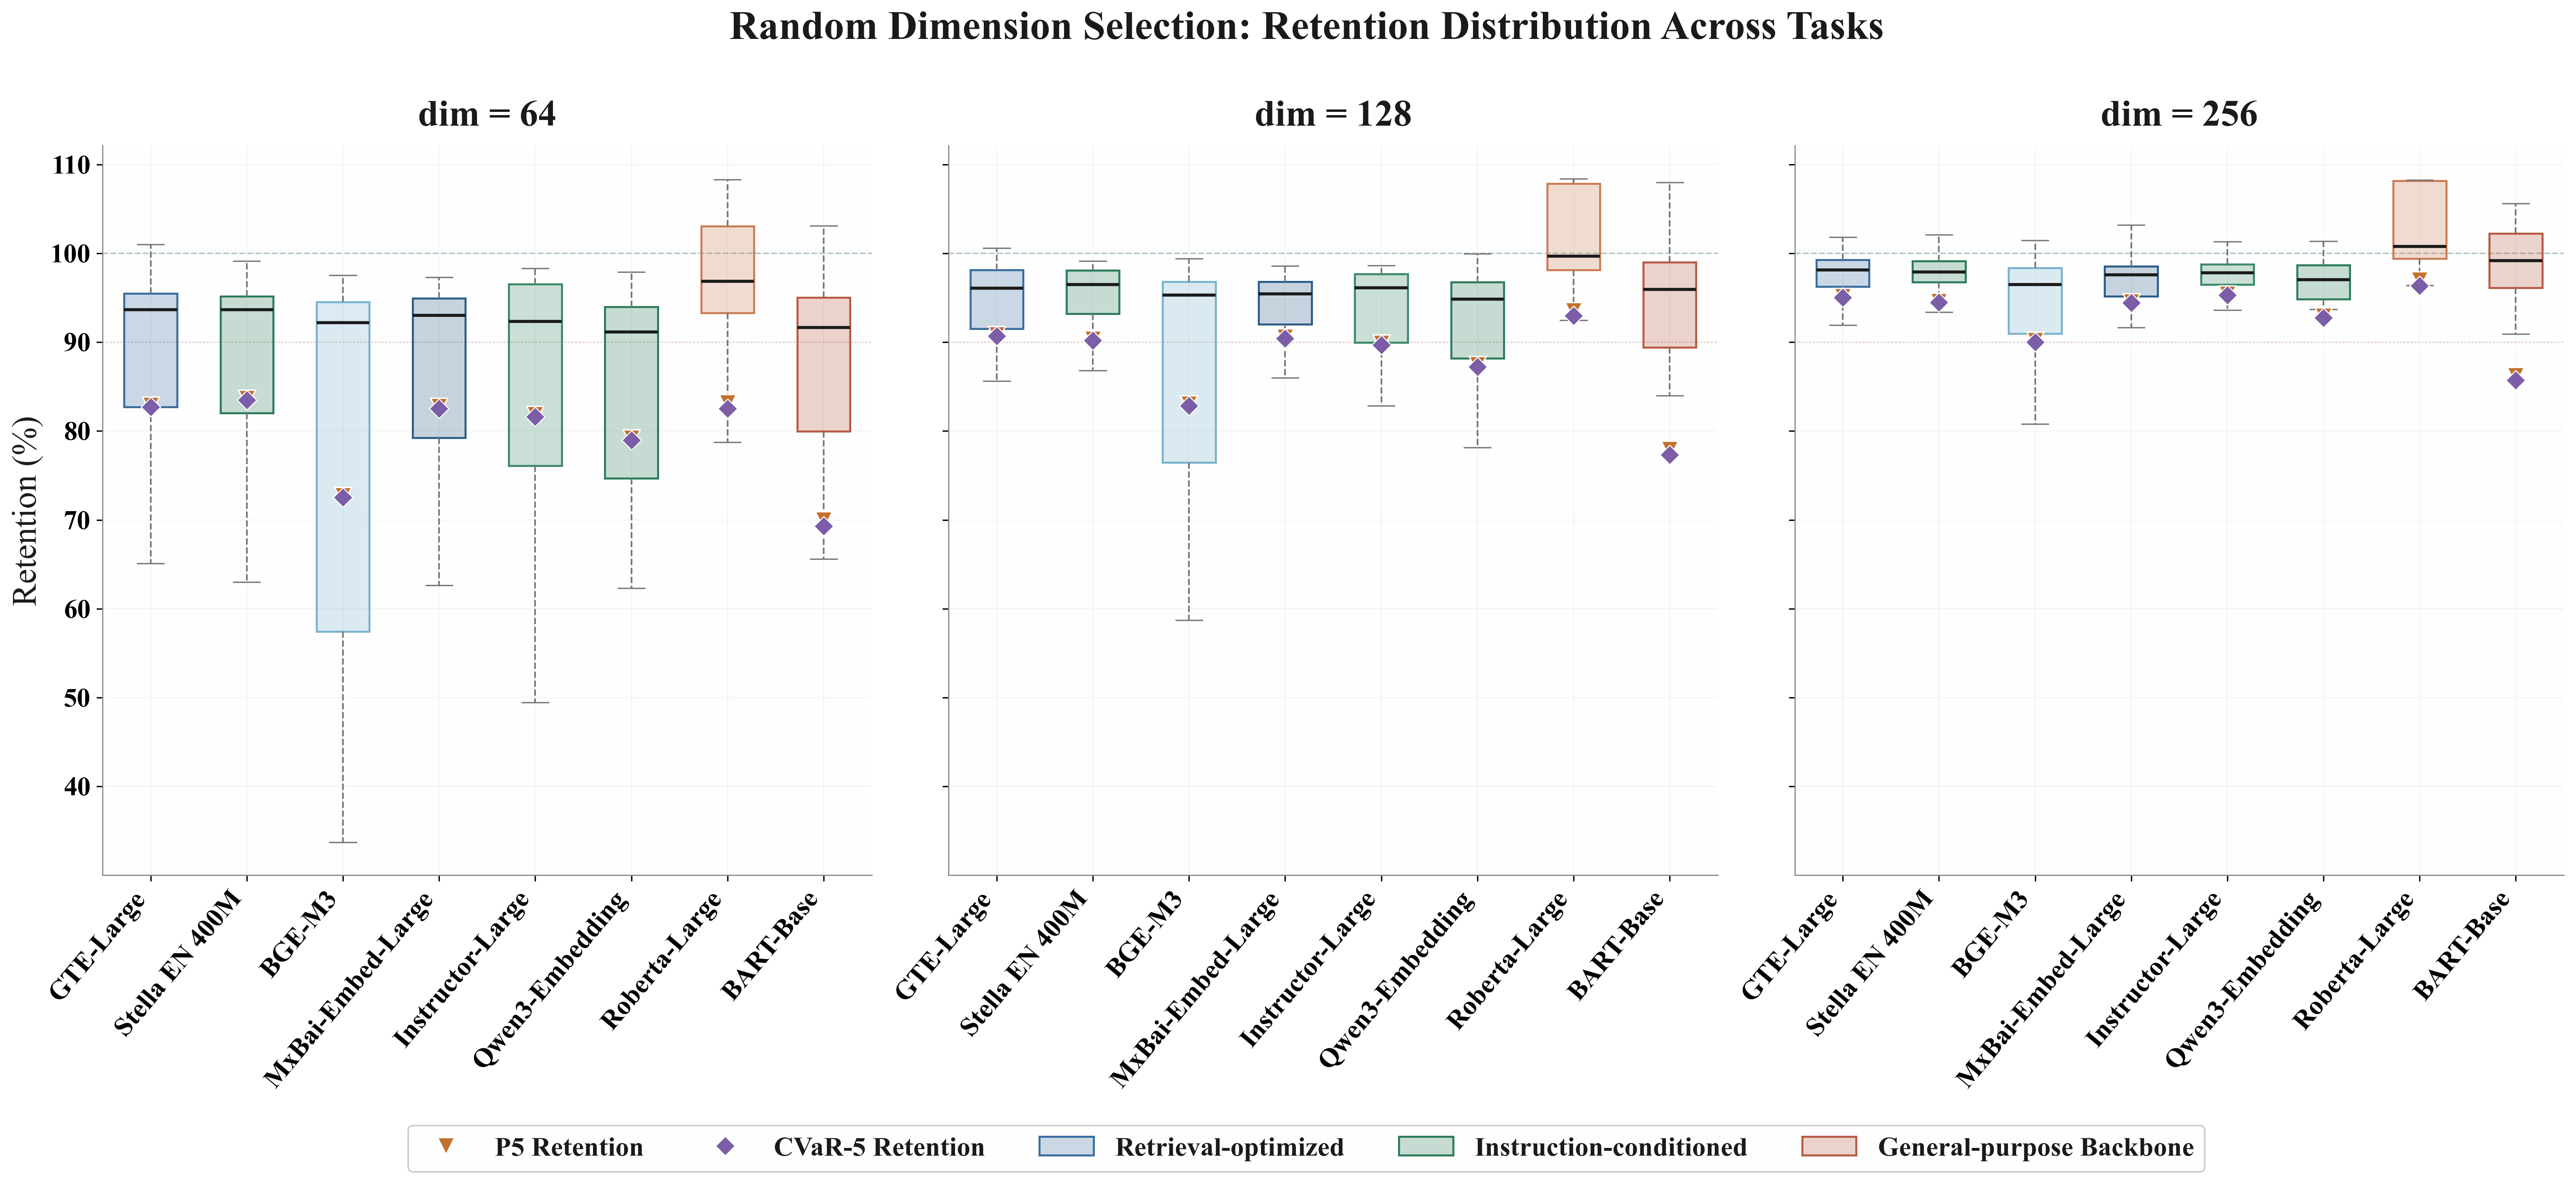
\includegraphics[width=0.95\linewidth]{figures/fig_random_variance.png}
    \caption{Retention distributions under random dimension selection across tasks. Each box plot shows the task-level spread of mean retention for retained dimensions $\in$ {64, 128, 256}. Triangle markers ($\triangle$) indicate P5 retention; diamond markers ($\diamond$) indicate CVaR-5 retention. Tail risk increases sharply as the retained dimension decreases.}
    \label{fig:random_variance_app}
\end{figure*}

\section{Leave-One-Out Importance Analysis}
\label{sec:loo}

Table~\ref{tab:importance_agreement} reports model-level Spearman correlation between standalone and alternative importance definitions and mean entropy per definition. Table~\ref{tab:loo_detailed} further shows per-task the results on Roberta-Large. The weak correlation between standalone and Leave-One-Out/marginal/Shapley importance confirms that chunk importance is inherently context-dependent. Standalone entropy is near-maximum (0.985--1.000) while Shapley entropy is substantially lower (0.655--0.933), revealing that interaction-aware importance detects much more structure. For STSBenchmark, LOO entropy drops to 0.343, indicating that some chunks are crucial in context even though they appear unimportant in isolation.

\begin{table*}[h]
    \centering
    \caption{Spearman correlation between standalone and alternative importance definitions (chunk size=4, retained dimension=256), and mean entropy per definition.}
    \label{tab:importance_agreement}
    \small
    \resizebox{\textwidth}{!}{%
    \begin{tabular}{lccccccc}
        \toprule
        & \multicolumn{3}{c}{Correlation with Standalone} & \multicolumn{4}{c}{Entropy} \\
        \cmidrule(lr){2-4} \cmidrule(lr){5-8}
        Model & LOO & Marginal & Shapley & Standalone & LOO & Marginal & Shapley \\
        \midrule
        GTE-Large & 0.094 & 0.155 & 0.132 & 0.999 & 0.936 & 0.939 & 0.625 \\
        BGE-M3 & 0.175 & 0.251 & 0.181 & 0.998 & 0.932 & 0.939 & 0.597 \\
        Stella EN 400M & 0.124 & 0.209 & 0.157 & 0.999 & 0.918 & 0.944 & 0.610 \\
        Roberta-Large & 0.091 & 0.296 & 0.235 & 0.997 & 0.838 & 0.891 & 0.660 \\
        Roberta-InBedder & 0.096 & 0.248 & 0.179 & 0.997 & 0.888 & 0.927 & 0.654 \\
        \bottomrule
    \end{tabular}%
    }
\end{table*}

\begin{table*}[h]
    \centering
    \caption{Per-task importance definition comparison for Roberta-Large (chunk size=4, retained dimension=256). Spearman correlations and normalized entropy for standalone, Leave-one-out, marginal, and Shapley importance. Low standalone-to-alternative correlations confirm importance is context-dependent.}
    \label{tab:loo_detailed}
    \small
    \resizebox{\textwidth}{!}{%
    \begin{tabular}{lcccccccc}
        \toprule
        & \multicolumn{4}{c}{Spearman $\rho$ with Standalone} & \multicolumn{4}{c}{Normalized Entropy} \\
        \cmidrule(lr){2-5} \cmidrule(lr){6-9}
        Task & LOO & Marginal & Shapley & $p$ (best) & Standalone & LOO & Marginal & Shapley \\
        \midrule
        ImdbClassification & $-$0.080 & 0.252 & 0.176 & $<$0.001 & 1.000 & 0.943 & 0.942 & 0.707 \\
        Banking77Classification & $-$0.001 & 0.078 & 0.156 & 0.012 & 0.996 & 0.949 & 0.914 & 0.860 \\
        TwentyNewsgroupsClustering & $-$0.038 & 0.137 & 0.132 & 0.029 & 0.998 & 0.922 & 0.950 & 0.932 \\
        MedrxivClusteringS2S & 0.018 & 0.039 & 0.073 & 0.247 & 0.999 & 0.952 & 0.945 & 0.842 \\
        STSBenchmark & 0.387 & 0.704 & 0.412 & $<$0.001 & 0.998 & 0.343 & 0.677 & 0.655 \\
        BIOSSES & 0.260 & 0.568 & 0.459 & $<$0.001 & 0.985 & 0.921 & 0.920 & 0.783 \\
        \bottomrule
    \end{tabular}%
    }
\end{table*}

\section{Train-Test Split Validation}
\label{sec:train_test_split}

Table~\ref{tab:train_test_split} reports the full train/test split results. Several patterns emerge from this analysis. The holdout gap is consistently positive across all models (74.5--87.2\% win rate), confirming that optimized selection does not merely overfit the ranking data and the selected dimensions genuinely generalize. The advantage remains modest for Retrieval-optimized Embedders and most Instruction-conditioned Embedders, but Roberta-InBedder and General-purpose Language Model Backbones show larger gain. These results validate the main paper's findings while addressing a key methodological concern: optimized selection does generalize to held-out data, and the paradigm-dependent gap is not an artifact of evaluating on the same data.

\begin{table}[t]
    \centering
    \small
    \caption{Train/test split experiment: Optimized dimension selection advantage evaluated on held-out data. Each MTEB task's test set is split 70\%/30\%: chunks are ranked on 70\% (train) and optimized performance is evaluated on the unseen 30\% (holdout). \textbf{Holdout Gap} = optimized $-$ random in this experiment. \textbf{Same-Data Gap} same-data optimized-random gap $-$ holdout optimized-random gap.}
    \label{tab:train_test_split}
    \resizebox{\columnwidth}{!}{%
    \begin{tabular}{@{}lccc@{}}
    \toprule
    \textbf{Model} & \textbf{Holdout Gap} & \textbf{Win\%} & \textbf{Same-Data Gap} \\
    \midrule
    \multicolumn{4}{l}{\textit{Retrieval-optimized Embedders}} \\
    GTE-Large & 1.74\% & 74.5\% & 0.67\% \\
    BGE-M3 & 2.70\% & 79.9\% & 1.91\% \\
    MxBai-Embed-Large & 1.69\% & 75.0\% & 0.90\% \\
    \midrule
    \multicolumn{4}{l}{\textit{Instruction-conditioned Embedders}} \\
    Roberta-InBedder & 4.02\% & 81.3\% & 4.17\% \\
    Qwen3-Embedding & 2.42\% & 77.3\% & 2.88\% \\
    Stella EN 400M & 2.21\% & 80.5\% & 1.01\% \\
    Instructor-Large & 1.52\% & 71.4\% & 1.37\% \\
    \midrule
    \multicolumn{4}{l}{\textit{General-purpose Language Model Backbones}} \\
    Roberta-Large & 5.15\% & 87.2\% & 6.60\% \\
    BART-Base & 4.26\% & 81.8\% & 5.82\% \\
    \midrule
    \textbf{Overall} & 2.86\% & 78.8\% & 2.82\% \\
    \bottomrule
    \end{tabular}%
    }
\end{table}

\section{Retrieval system cost}
\label{sec:retrieval_cost}
Using FAISS FlatIP, Random-256 retains 87.5--98.4\% of full-dim nDCG while reducing raw vector storage by 4$\times$ (Table~\ref{tab:retrieval_cost}). Random projection is included as a projection-based comparator, but it requires applying a projection matrix. For GTE-Large, Random-256 reduces P50 latency from 0.16--0.23ms to 0.04--0.08ms, a 2.9--4.3$\times$ speedup.

\begin{table}[t]
    \centering
    \caption{Retrieval cost--quality tradeoff at dim=256 for GTE-Large using FAISS FlatIP. nDCG@10 and Recall report retention relative to the full-dimensional baseline for each task.}
    \label{tab:retrieval_cost}
    \resizebox{\columnwidth}{!}{%
    \begin{tabular}{llcccc}
        \toprule
        Task & Method & nDCG@10 & Mem (MB) & Latency (ms) & Recall \\
        \midrule
        \multirow{3}{*}{NFCorpus} & Full-1024 & 100.0\% & 14.2 & 0.16 & 100.0\% \\
        & Random-256 & 98.4\% & 3.5 & 0.04 & 96.7\% \\
        & RP-256 & 85.3\% & 3.5 & 0.38 & 82.9\% \\
        \midrule
        \multirow{3}{*}{ArguAna} & Full-1024 & 100.0\% & 19.5 & 0.22 & 100.0\% \\
        & Random-256 & 93.7\% & 4.9 & 0.05 & 95.9\% \\
        & RP-256 & 94.0\% & 4.9 & 0.40 & 93.8\% \\
        \midrule
        \multirow{3}{*}{SciFact} & Full-1024 & 100.0\% & 19.5 & 0.23 & 100.0\% \\
        & Random-256 & 87.5\% & 4.9 & 0.08 & 93.8\% \\
        & RP-256 & 83.4\% & 4.9 & 0.80 & 88.1\% \\
        \bottomrule
    \end{tabular}%
    }
\end{table}


\end{document}
